%---------------------Settings---------------------------%
\documentclass[10pt,a4paper,twocolumn,twoside,UTF8]{article}
\usepackage{geometry}
	\geometry{left=1.8cm,right=1.8cm,top=2.5cm,bottom=2cm}
% \usepackage{xeCJK}
\usepackage{amsmath,paralist,enumitem,booktabs,multirow,graphicx,subfig,setspace,listings,multicol,lettrine}
	\setlength{\parindent}{2em}
	\lstset{language=Python}
\usepackage{fancyhdr}
\usepackage{layout}
\setlength\columnsep{0.8cm}

%%begin----------Set header and footer----------------%%
\usepackage{ifthen}
\newboolean{first}
\setboolean{first}{true}
\pagestyle{fancy}
	\fancypagestyle{maincontent}{
		\fancyhf{}  
		\fancyhead[EL, OR]{\thepage}
		\fancyhead[EC]{C6 Optical properties and applications of optical fibers}
		\fancyhead[OC]{GENERAL PHYSICS LABORATORY}
		\renewcommand\headrulewidth{0pt}
	}
	
	\usepackage{datetime}
	\fancypagestyle{firstpage}{
		\setboolean{first}{false}
		\fancyhf{}  
		\fancyhead[L]{Sun Yat-sen University}
		\fancyhead[R]{\shortmonthname[\the\month], \the\year}
		\fancyhead[C]{
		          \large{GENERAL PHYSICS LABORATORY}
		          }
	}
	
	\newcommand{\makefirstpageheadrule}{
	\makebox[0pt][s]{\rule[0.6\baselineskip]{\headwidth}{0.3pt}}
	\makebox[0pt][s]{\protect\hspace{-0.34em}\rule[0.75\baselineskip]{\headwidth}{0.3pt}}
	\protect\vspace{-20pt}
	}

	\newcommand{\makeheadrule}{
	\makebox[0pt][l]{\rule[1\baselineskip]{\headwidth}{0.3pt}}
	\protect\vspace{-20pt}
	}

	\renewcommand{\headrule}{
	\ifthenelse{\boolean{first}}{\makeheadrule}
	{\makefirstpageheadrule}
	}
%%end--------------Set header and footer-----------%%

%%begin-----------------Reference-----------------------%%
\usepackage[colorlinks,linkcolor=blue,urlcolor=blue,citecolor=blue]{hyperref}
\usepackage[hyperref=true,backend=biber,bibstyle=gb7714-2015,citestyle=numeric-comp,sorting=none,backref=true]{biblatex}
\addbibresource{REF.bib}
%%end-------------------Reference-----------------------%%

%end---------------------Settings---------------------------%




%%%%%%%%%%%%%%%%%%%%%%%%%%%%%%%%%%%%%%%%%%%%%%%%%%%%%%%%%%
%%%%%%%%%%%%%%%%%%%%%%%%%Document%%%%%%%%%%%%%%%%%%%%%%%%%
%%%%%%%%%%%%%%%%%%%%%%%%%%%%%%%%%%%%%%%%%%%%%%%%%%%%%%%%%%

%%begin-------------------Abstract-----------------------%%
\begin{document}
\title{\LARGE\textbf{Optical properties and applications of optical fibers} \footnotemark[1]}
\author{\large\textit{Ziwei, Huang}$^{1}$\footnotemark[2]
\\ \normalsize{1 Zhongshan School of Medicine, Sun Yat-sen University, Guangzhou  { \rm 510275}, China}}
\date{}

\twocolumn[
	\begin{@twocolumnfalse}
	\maketitle  
	\renewcommand{\abstractname} {} 
	\begin{abstract}
	\vspace{-3em}
	{\bf Abstract: }
	{\small 
    Optical fiber is fundamental to modern communication systems and essential for a wide range of technologies such as fiber-optic-based sensors. 
	It is of great importance to understand the mechanism of optical fiber transmission. 
	The specific objective of this study was to investigate the optical properties of optical fiber and its broad application prospects in high-precision sensors. 
	We first built a source-fiber coupling system and adjusted the position of the fiber to get the highest coupling efficiency. 
	We then investigated the numerical apertures and characteristics of the exit spots of fibers with different diameters. 
	We found that fibers with higher diameters tended to have larger numerical apertures, and their exit spots were generally more diffused, while fibers with lower diameters tended to have smaller numerical apertures, and their exit spots generally showed a concentrated pattern with high light intensity in the center and a blurred edges. 
	We also investigated the change of the polarization state when the light passed through a fiber. 
	Unfortunately, due to the limitations of our instruments, the fluctuation of the output luminous power was so great that we could not make an accurate observation; thus, this question still remains unsolved. 
	Finally, we developed a strain sensor and a temperature sensor based on the optical fiber-based Mach-Zehnder interferometer, which have reached high precision in measuring.
	}
	\par
	\textbf{Keywords: Optical fiber, Source-fiber coupling, Numerical aperture, Polarization state, Stocks parameters,Optical-fiber-based Mach-Zehnder interferometer, Temperature sensor, Strain sensor} 
	\vspace{2em}
	\end{abstract}
	\end{@twocolumnfalse}
]

\renewcommand{\thefootnote}{\fnsymbol{footnote}}
\footnotetext[1]{Supported and taught by Luyoutang, School of Physics, Sun Yat-sen University}
\footnotetext[2]{Corresponding author. ID: 20980066 Email: \url{huangzw29@mail2.sysu.edu.cn} }
%%end-------------------Abstract-----------------------%%

\thispagestyle{firstpage} 
\pagestyle{maincontent}

%%begin-------------------Intro-----------------------%%
\section{Introduction}
\lettrine[lines=2]{T}{he} past decade has seen the rapid development of optical fiber. 
Optical fibers are transparent and flexible fibers made up of plastic or glass and basically composed of two coaxial layers: core and cladding. 
It can carry information in the form of light pulses from one end of the fiber to another with an impressively low transmission loss and thus plays a vital role in modern communication systems. 
Furthermore, since the optical properties of the fiber are sensitive to changes in the environment, they have been widely used in the field of high-precision sensing. 
Investigating the optical properties and prospective applications of optical fibers are essential in optical fiber optics. 
In this thesis we focused on the major optical properties of the optical fiber including the coupling efficiency, numerical aperture and its effect on the polarization state of the light. 
We also investigated how the optical fibers responded to changes of the environment factors such as temperature and strain, and basing on these properties we developed high-precision strain and temperature sensors basing on the optical-fiber-based Mach-Zehnder interferometer.

%%end-------------------Intro-----------------------%%
% \newpage % Change the column
%%begin-----------------Method-----------------------%%
\section{Experimental principles and method}
	\subsection{Experimental principle\autocite{shenGeneralPhysicsLaboratory2015}}
		\subsubsection{The optical fiber}
		Optical fibers are transparent and flexible fibers made up of plastic or glass and basically composed of two coaxial layers: core and cladding. 
		A typical structure of the optical fiber is illustrated in Fig. \ref{fig.illus-1.1}. 
		\begin{figure}[htbp]
			\centering
			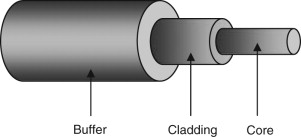
\includegraphics[width=0.4\textwidth]{attachments/illus-1.1.png}
			\caption{\textbf{A typical structure of the optical fiber}}
			\label{fig.illus-1.1}
		\end{figure}
		
		Optical fibers can be classified in different way. 
		For example, based on the refractive index, they can be classified into:
		\paragraph{A. Step Index Fibers:} The refractive index of the core of the optical fiber is uniform, so the light goes in a straight line in the fiber.
		\paragraph{B. Graded Index Fibers:} The refractive index of the core of the optical fiber decreases as the radial distance from the fiber axis increases, thus the light goes in a curve line in the fiber.
		
		Or, based on the mode of propagation of light:
		\paragraph{A. Single-Mode Fibers:} These fibers can transfer only one specific type of mode. They generally have a smaller diameter and better performance, thus suitable for long-distance transmission of signals.
		\paragraph{B. Multi-mode Fibers:} These fibers can transfer multiple modes simultaneously. They generally have a greater diameter and lower  performance, thus suitable for short-distance transmission of signals.

		A more exact distinction between single-mode fibers and multi-mode fibers are quantified by the normalized frequency defined as (Eq. \ref{eq.1}):
		\begin{equation}
			\nu = \frac{2\pi a n_1\sqrt{(2\frac{n_1-n_2}{n_1})}}{\lambda}
			\label{eq.1}
		\end{equation}
		$a$ is the diameter of the fiber, $\lambda$ is the wavelength of the light, $n_1$ is the refractive index of the core and $n_2$ is the refractive index of the cladding.
		
		Generally, if $\nu$ is lower than around $2.4$, the fiber is likely a single-mode fiber. Otherwise, it is usually a multi-mode fiber with a total number of modes varying from $\frac{\nu^2}{4}$ to $\frac{\nu^2}{2}$.
		
		The transmission patterns of light within different types of fibers are illustrated in Fig. \ref{fig.illus-1.2}
		\begin{figure}[htbp]
			\centering
			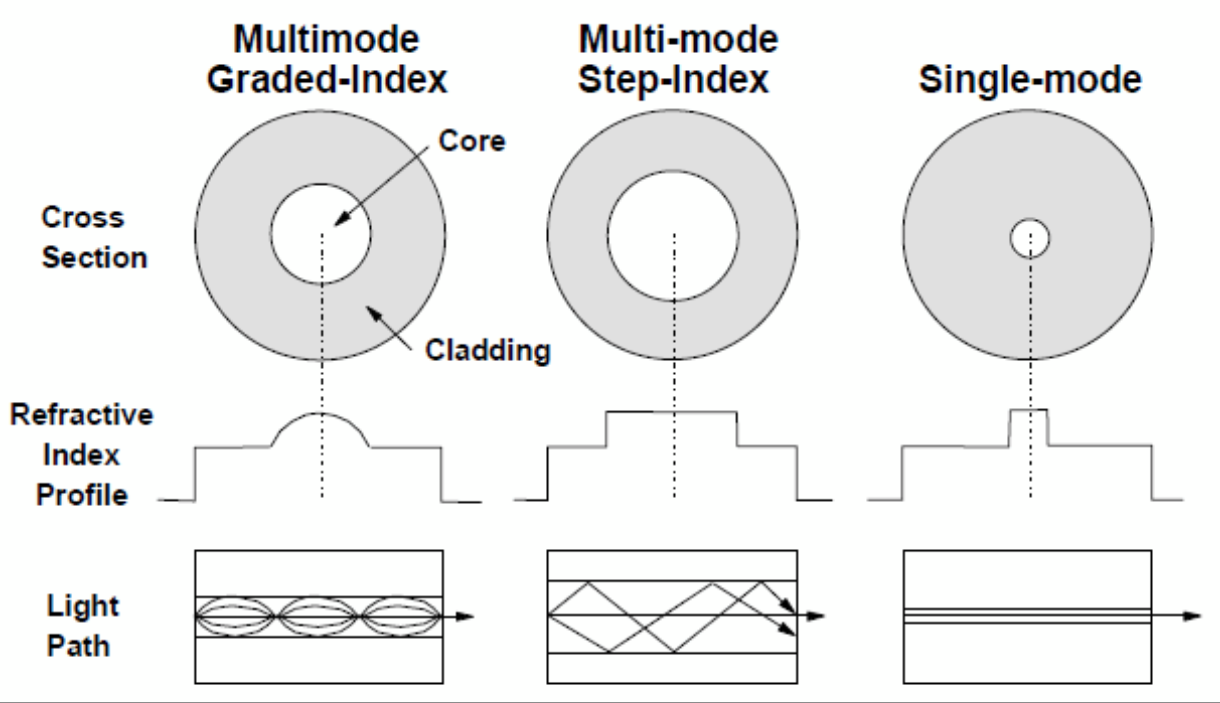
\includegraphics[width=0.4\textwidth]{attachments/illus-1.2.png}
			\caption{\textbf{The transmission pattern of light in fibers}}
			\label{fig.illus-1.2}
		\end{figure}

		\subsubsection{Numerical aperture of the fiber}
		According to the principle of total internal reflection, to guarantee successful light transmission, 
		the refractive index $(n)$ of the core must be greater than that of the cladding and the angle of incidence $\theta_0$ must be restricted in a specific range (Fig. \ref{fig.illus-2.1}). 
		The maximum permissible $\theta_0$ is determined by Eq. \ref{eq.2.1}:
		\begin{align}
			n_0sin\theta_0 &= n_1sin(\frac{\pi}{2} - \theta_c) \notag \\
			&= \sqrt{n_1^2-n_2^2}
			\label{eq.2.1}
		\end{align}
		\begin{figure}[htbp]
			\centering
			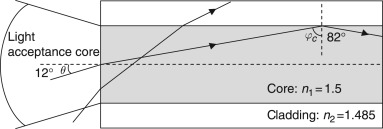
\includegraphics[width=0.4\textwidth]{attachments/illus-2.1.png}
			\caption{\textbf{The angle of incidence}}
			\label{fig.illus-2.1}
		\end{figure}
		$n_0sin\theta_0$ is referred to as the numerical aperture of the fiber (NA). Obviously, the larger the numerical aperture of the fiber, the easier it is to couple the fiber, and the transmission energy should be higher.
		
		A convenient method to measure the numerical aperture is measuring the diameter $d$ of the output distant field facula in given distances $l$ from the end face of the fiber (Fig. \ref{fig.illus-2.2}). 
		The numerical aperture can be calculated as (Eq. \ref{eq.2.2}):
		\begin{align}
			NA &= n_0sin\theta_0 \notag \\
			   &= n_1\sqrt{2\Delta} \label{eq.2.2} \\
			where: \Delta &= \frac{n_1-n_2}{n_1} \notag
		\end{align}
		\begin{figure}[htbp]
			\centering
			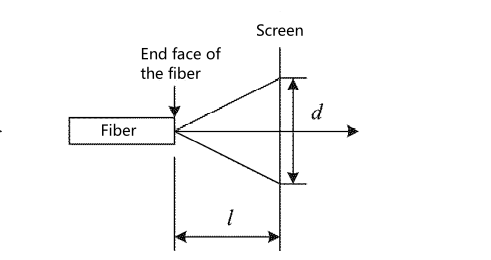
\includegraphics[width=0.4\textwidth]{attachments/illus-2.2.png}
			\caption{\textbf{Distant field facula method}}
			\label{fig.illus-2.2}
		\end{figure}

		\subsubsection{Source-fiber coupling}
		In fiber optic transmission systems, the optical signal power should be launched from a light source and accepted by an optical fiber. 
		This process is called the "source-fiber coupling". The most straightforward way is direct coupling without any other assistant instruments. 
		However, it is very difficult to adjust the fiber to the optimum position, and the coupling efficiency is limited as a result of the diffusion of the light. 
		To reduce coupling loss, a lens can be used to focus the light onto the face of the fiber.

		The coupling coefficient $\eta$ is determined by Eq. \ref{eq.3.1}, and the coupling loss $L$ measured in $dB$ is determined by Eq. \ref{eq.3.2}. 
		\begin{align}
			\eta &= \frac{P_1}{P_2} \times 100\% \label{eq.3.1} \\
			L   &= -10ln(\frac{P_2}{P_1}) \label{eq.3.2} 
		\end{align}
		$P_1$: Transmission luminous power in the fiber. $P_2$: Output luminous power of the laser.

		\subsubsection{Description of the polarization state: Stokes parameters}
		The classical description of polarized light is the polarization ellipse, which provides complete information, including amplitude and orientation. 
		However, it is technically impossible to measure the polarization ellipse directly through an experiment. 
		An equivalent description is the Stokes polarization parameters introduced by George Gabriel Stokes in 1852 which includes four intensity parameters: $S = (S_0, S_1, S_2, S_3)$ .

		If we have a beam of polarized light whose polarization ellipse is:
		\begin{align}
			E_x	&= a_1cos\tau \\
			E_y	&= a_2cos(\tau+\delta)
				\label{eq.4.1}
	   	\end{align}
		We introduce two angles: the azimuth angle $\psi$ and the declination $\chi$, which are defined as:
		\begin{align}
			tan(2\psi)	&= tan(2\alpha) cos\delta \label{eq.4.2.1}\\
			tan(2\chi)  &= sin(2\alpha) sin\delta \label{eq.4.2.2}\\
			where: tan\alpha &= \frac{a_2}{a_1} \notag
		\end{align}
		We measure the following intensity:
		\begin{enumerate}[label=\arabic*.]
			\item Intensity of the light when the transmission axis of the analyzer is parallel to the coordinate axis: $I_x$ and $I_y$
			\item Intensity of the light when the transmission axis of the analyzer is along $\pm \frac{\pi}{4}$ from the x axis: $I_{+\frac{\pi}{4}}$ and $I_{-\frac{\pi}{4}}$
			\item Intensity of the light when we use a quarter wave plate to generate a right-rotated circularly polarized light and a left-rotated circularly polarized light: $I_R$ and $I_L$
		\end{enumerate}
		We get the following.
		\begin{align}
			S_0 &= I_x + I_y = a^2_1 + a^2_2 \label{eq.4.3.1}\\
			S_1 &= I_x-I_y = a^2_1-a^2_2 \label{eq.4.3.2}\\
			S_2 &= I_{+\frac{\pi}{4}} - I_{-\frac{\pi}{4}} = 2 a_1 a_2cos\delta \label{eq.4.3.3}\\
			S_3 &= I_L-I_R = 2a_1 a_2 sin\delta \label{eq.4.3.4}
		\end{align}
   		
		Then, the Stokes polarization parameters can be defined as follows.
		\begin{align}
			S^2_0 &= S^2_1 + S^2_2 + S^2_3  \label{eq.4.4.1}\\
			S_1 &= S_0 cos2\chi cos2\psi  \label{eq.4.4.2}\\
			S_2 &= S_0 cos2\chi sin2\psi  \label{eq.4.4.3}\\
			S_3 &= S_0 sin2\chi  \label{eq.4.4.4}
		\end{align}

		An alternative simpler method to measure the Stokes parameters is to measure the following intensity:
		\begin{enumerate}[label=\arabic*.]
			\item Intensity of the light when the transmission axis of the analyzer is parallel to the coordinate axis: $I_x$ and $I_y$
			\item Intensity of the light when the transmission axis of the analyzer is along $+ \frac{\pi}{4}$ from the x axis: $I_{+\frac{\pi}{4}}$ 
			\item Intensity of the light when use a quarter wave plate to generate a right-rotated circularly polarized light: $I_R$
		\end{enumerate}
		Then, the Stokes polarization parameters can be calculated by:
		\begin{align}
			S_0 &= P_x + P_y  \label{eq.4.5.1}\\
			S_1 &= P_x - P_y  \label{eq.4.5.2}\\
			S_2 &= 2P_{+\frac{\pi}{4}} - S_0  \label{eq.4.5.3}\\
			S_3 &= S_0 - 2P_R  \label{eq.4.5.4}\\
		\end{align}

		Obviously, $S_0$ can be interpreted as a point on a sphere with radius $r=S_0$, and its coordinates are $(S_1, S_2, S_3)$. 
		This sphere is referred as the Poincare sphere Fig. \ref{fig.illus-3.1}, any point on which represents a state of polarization.
		\begin{figure}[htbp]
			\centering
			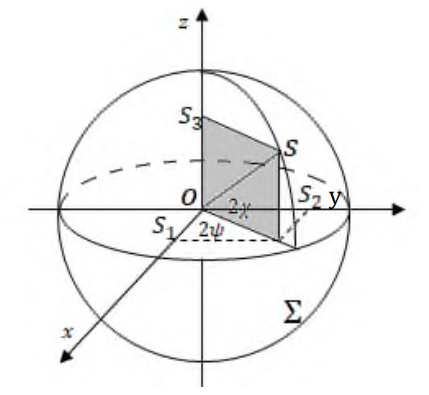
\includegraphics[width=0.4\textwidth]{attachments/illus-3.1.png}
			\caption{\textbf{The Poincare sphere}}
			\label{fig.illus-3.1}
		\end{figure}

		The polarization state can also represented by the Stocks vector defined as: 
		\begin{equation}
			S=(S_0, S_1, S_2, S_3)^T
			\label{eq.4.6}
		\end{equation}
		For example, the horizontal polarized light($LHP$) and the vertical polarized light($LVP$) can be represented as:
		\begin{equation*}
		S_{LHP} = 
			\begin{bmatrix}
				1 \\
				1 \\
				0 \\
				0 \\
			\end{bmatrix}, \
		S_{LVP} = 
			\begin{bmatrix}
				1 \\
				-1 \\
				0 \\
				0 \\
			\end{bmatrix}
		\end{equation*}
		\subsubsection{Optical-fiber-based Mach-Zehnder interferometer}
		One typical optical-fiber-based Mach-Zehnder interferometer is illustrated as Fig. \ref{fig.illus-4.1}. 
		The laser is injected into the fiber and split into two coherent light. 
		The two branches of light travel through two fibers, respectively, and finally meet at the combiner, at which the interference happens and the interference pattern is captured by the photodetector. 
		According to the principle of interference, the intensity $I$ is determined by the optical phase difference $\delta$ (Eq. \ref{eq.5.1}).
		\begin{figure}[htbp]
			\centering
			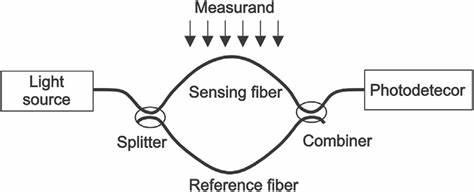
\includegraphics[width=0.4\textwidth]{attachments/illus-4.1.png}
			\caption{\textbf{Optical-fiber-based Mach-Zehnder interferometer}}
			\label{fig.illus-4.1}
		\end{figure}
		
		\begin{equation}
			I \propto 1+cos\delta
			\label{eq.5.1}
		\end{equation}
		If the optical phase difference $\delta$ changes, the interference fringes will shift correspondingly. By counting the number of shifted interference fringes, it's possible to infer the changes of $\delta$. 

		\subsubsection{Strain sensor and temperature sensor basing on the optical-fiber-based Mach-Zehnder interferometer}
		Taking advantages of the agile and precise response of the shift of the interference fringes to the change of the optical path difference $\Delta \phi$, high-precision sensor can be developed basing on the optical-fiber-based Mach-Zehnder interferometer. 
		As illustrated in Fig. \ref{fig.illus-4.1}, one of the two fibers is set as the "reference fiber", and the measurand is exerted on the other (referred to as the "sensing fiber"). Any change of the measurand will result in change of the optical path in the sensing fiber, causing shift of the interference fringes.
		\paragraph{A. Strain sensor:}~
		\newline 
		\indent
		When the strain exerted on the sensing fiber changes, the optical path difference can be expressed as
		\begin{equation}
			\Delta \phi = \beta \Delta L+ L\Delta \beta
			\label{eq.6.1}
		\end{equation}
		Where $\beta \Delta L$ represents the elongation of the light path, and the $L\Delta \beta$ represents the strain light effect and the waveguide mode dispersion.

		\paragraph{B. Temperature sensor:}~
		\newline 
		\indent
		When the temperature changes, the optical path difference can be expressed as
		\begin{equation}
			\Delta \phi = \frac{2\pi}{\lambda} \Delta T(\frac{n}{L}\frac{dL}{dT}+ \frac{dn}{dT})
			\label{eq.6.2}
		\end{equation}
		Where $\frac{dL}{dT}$ represents the effect of the linear thermal expansion of the fiber, and the $\frac{dn}{dT}$ represents change of refractive index.

	\subsection{Major instruments and materials}
	\subsubsection{Optical fibers}
	Optical fibers used in this paper include one multi-mode fiber with a diameter of $\phi \ 62.5\mu m$ and two single-mode fibers with diameters of $\phi \ 4\mu m$  and $\phi \ 9\mu m$ . 
	All fibers are assembled with FC/PC connectors.
	\subsubsection{Source-fiber coupling alignment jig}
	The structure is illustrated in Fig. \ref{fig.illus-5.1}. The alignment jig allows for five-dimensional adjustment, which promises the precision of coupling.
	\begin{figure}[htbp]
		\centering
		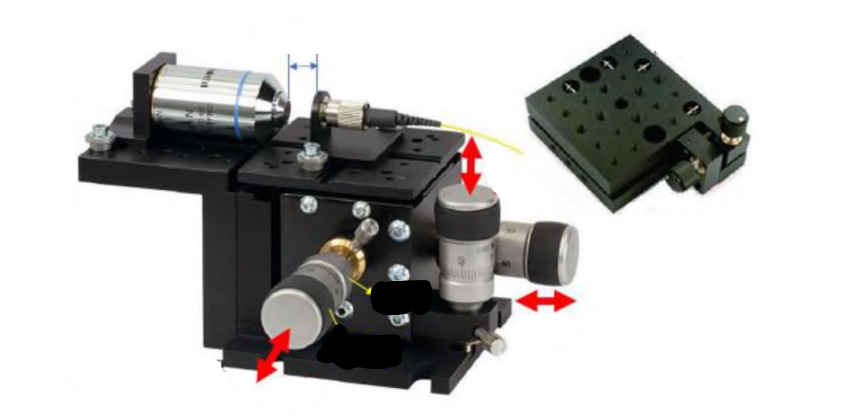
\includegraphics[width=0.4\textwidth]{attachments/illus-5.1.png}
		\caption{\textbf{Source-fiber coupling alignment jig}}
		\label{fig.illus-5.1}
	\end{figure}

	\subsubsection{Optical fiber information experimental system}
	The core component of the optical fiber information experimental system used in this study is illustrated in Fig. \ref{fig.illus-6.1}. 
	It is basically a Mach-Zehnder interferometer, but integrated with temperature and strain controllers which allows controlling the measurand conveniently. 
	When investigating the shift of the interference fringes responding to the change of the strain, the fiber integrated with temperature controller is set as the "reference fiber", and vise versa.
	\begin{figure}[htbp]
		\centering
		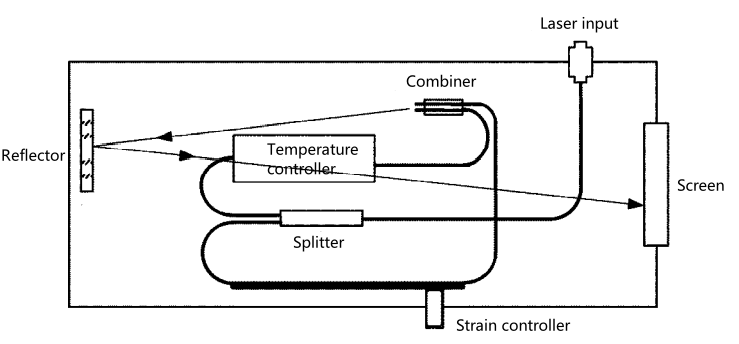
\includegraphics[width=0.4\textwidth]{attachments/illus-6.1.png}
		\caption{\textbf{Core component of the optical fiber information experimental system}}
		\label{fig.illus-6.1}
	\end{figure}
	
	\subsection{Method}
		\begin{enumerate}[label=\arabic*.]
			\item We first built an optical fiber coupling system and adjusted the position of the fiber to get the highest coupling efficiency. The coupling efficiency and coupling loss of the three fibers by direct coupling and coupling through a lens were measured to estimate the effect.
			\item Then we investigated the numerical apertures and characteristics of the exit spots of the three fibers.
			\item After that, the polarization states of the laser represented by the Stocks parameters were measured and compared before and after it passed through a fiber to investigate the influence of fiber transmission on the polarization state.
			\item Finally, we developed a strain sensor and a temperature sensor basing on optical-fiber-based Mach-Zehnder interferometer and investigated the shift of the interference fringes responding to the change of the strain and temperature.
		\end{enumerate}
%%end-------------------Method-----------------------%%

%%begin-------------------Result-----------------------%%
\section{Result}
	\subsection{Source-fiber coupling}
	The coupling efficiency and coupling loss of the three fibers were calculated according to Eq. \ref{eq.3.1} and Eq. \ref{eq.3.2} and shown as Tab. \ref{tab.1.1}
	\begin{table*}[htbp]
		\centering
			\begin{tabular}{llll}
				\toprule
				Fiber & ~ & Direct coupling & Through a lens \\
				\midrule
				$\phi 62.5\mu m$ & Coupling efficency(\%) & $0.301\pm0.004$ & $73.785\pm1.508$ \\
				~ & Coupling loss($dB$) & $58.057\pm0.142$ & $3.040\pm0.204$ \\
				\midrule
				$\phi 9\mu m$ & Coupling efficency(\%) & $0.0083\pm0.0003$ & $71.354\pm1.230$ \\
				~ & Coupling loss($dB$) & $94.000\pm0.386$ & $3.375\pm0.172$ \\
				\midrule
				$\phi 4\mu m$ & Coupling efficenc(\%) & $0.0031\pm0.0002$ & $44.583\pm1.262$ \\
				~ & Coupling loss($dB$) & $103.763\pm0.824$ & $8.078\pm0.283$ \\
				\bottomrule
			\end{tabular}
			\caption{\textbf{The coupling efficiency and coupling loss of the three fibers}}
			\label{tab.1.1}
	\end{table*}
	We found that compared to direct coupling, coupling through a lens gained a great improvement in reducing the coupling loss.
	The effectiveness is consistent in all three fibers, proving that coupling through a lens is an effective way to couple the light source and the fiber.
	
	\subsection{Numerical aperture}
	The facula patterns at $7.5 cm$ and the numerical apertures of the three fibers measured by distant-field-facula method are shown in Fig. \ref{fig.1}, and the results are summarized in Tab. \ref{tab.2.1}.
	
	We found that fiber a with higher diameter ($\phi 62.5\mu m$) tended to have a larger numerical aperture and the exit spot is generally more diffused, 
	while fibers with lower diameters ($\phi 9\mu m$ and $\phi 4\mu m$) tended to have smaller numerical apertures and their exit spots generally showed a concentrated pattern with high light intensity in the center and blurred edges.

	\begin{figure*}[htbp]
		\centering
		\subfloat[The numerical aperture. $\phi 62.5\mu m$]{\label{fig.1.1.1}
		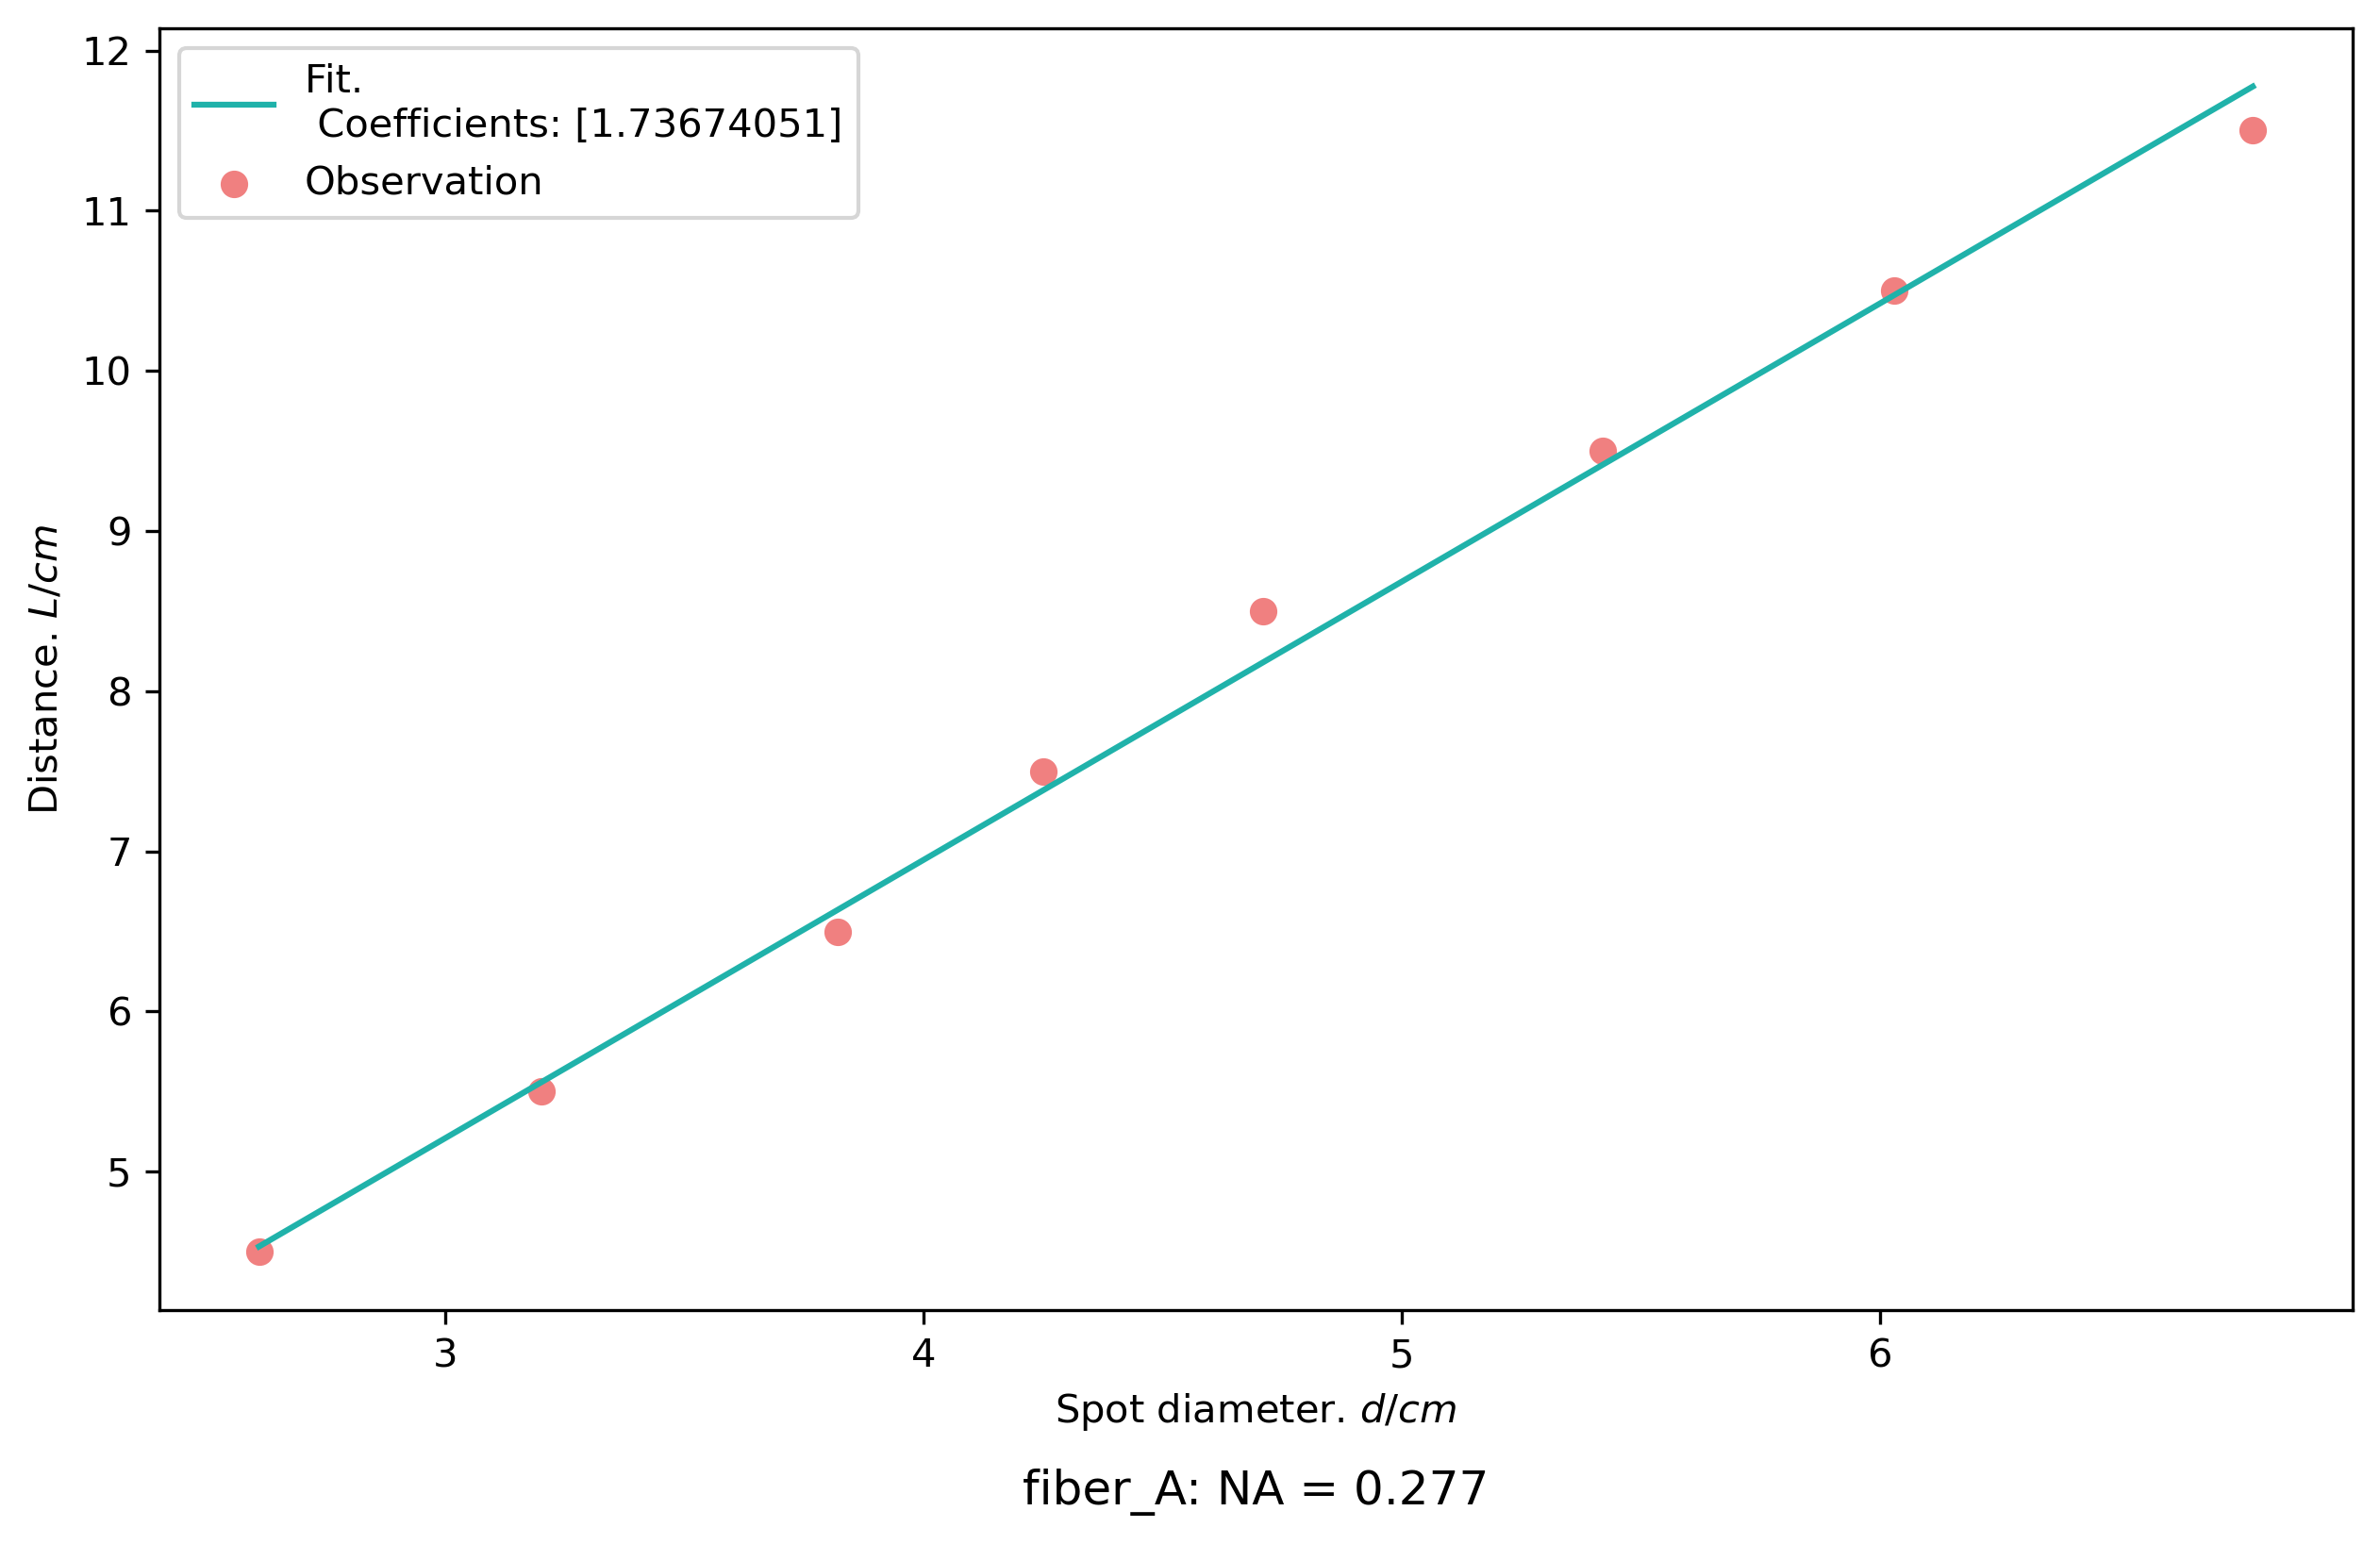
\includegraphics[width=0.3\textwidth]{attachments/fig.1.1.1.png}
		}
		\subfloat[The numerical aperture. $\phi 9\mu m$]{\label{fig.1.1.2}
		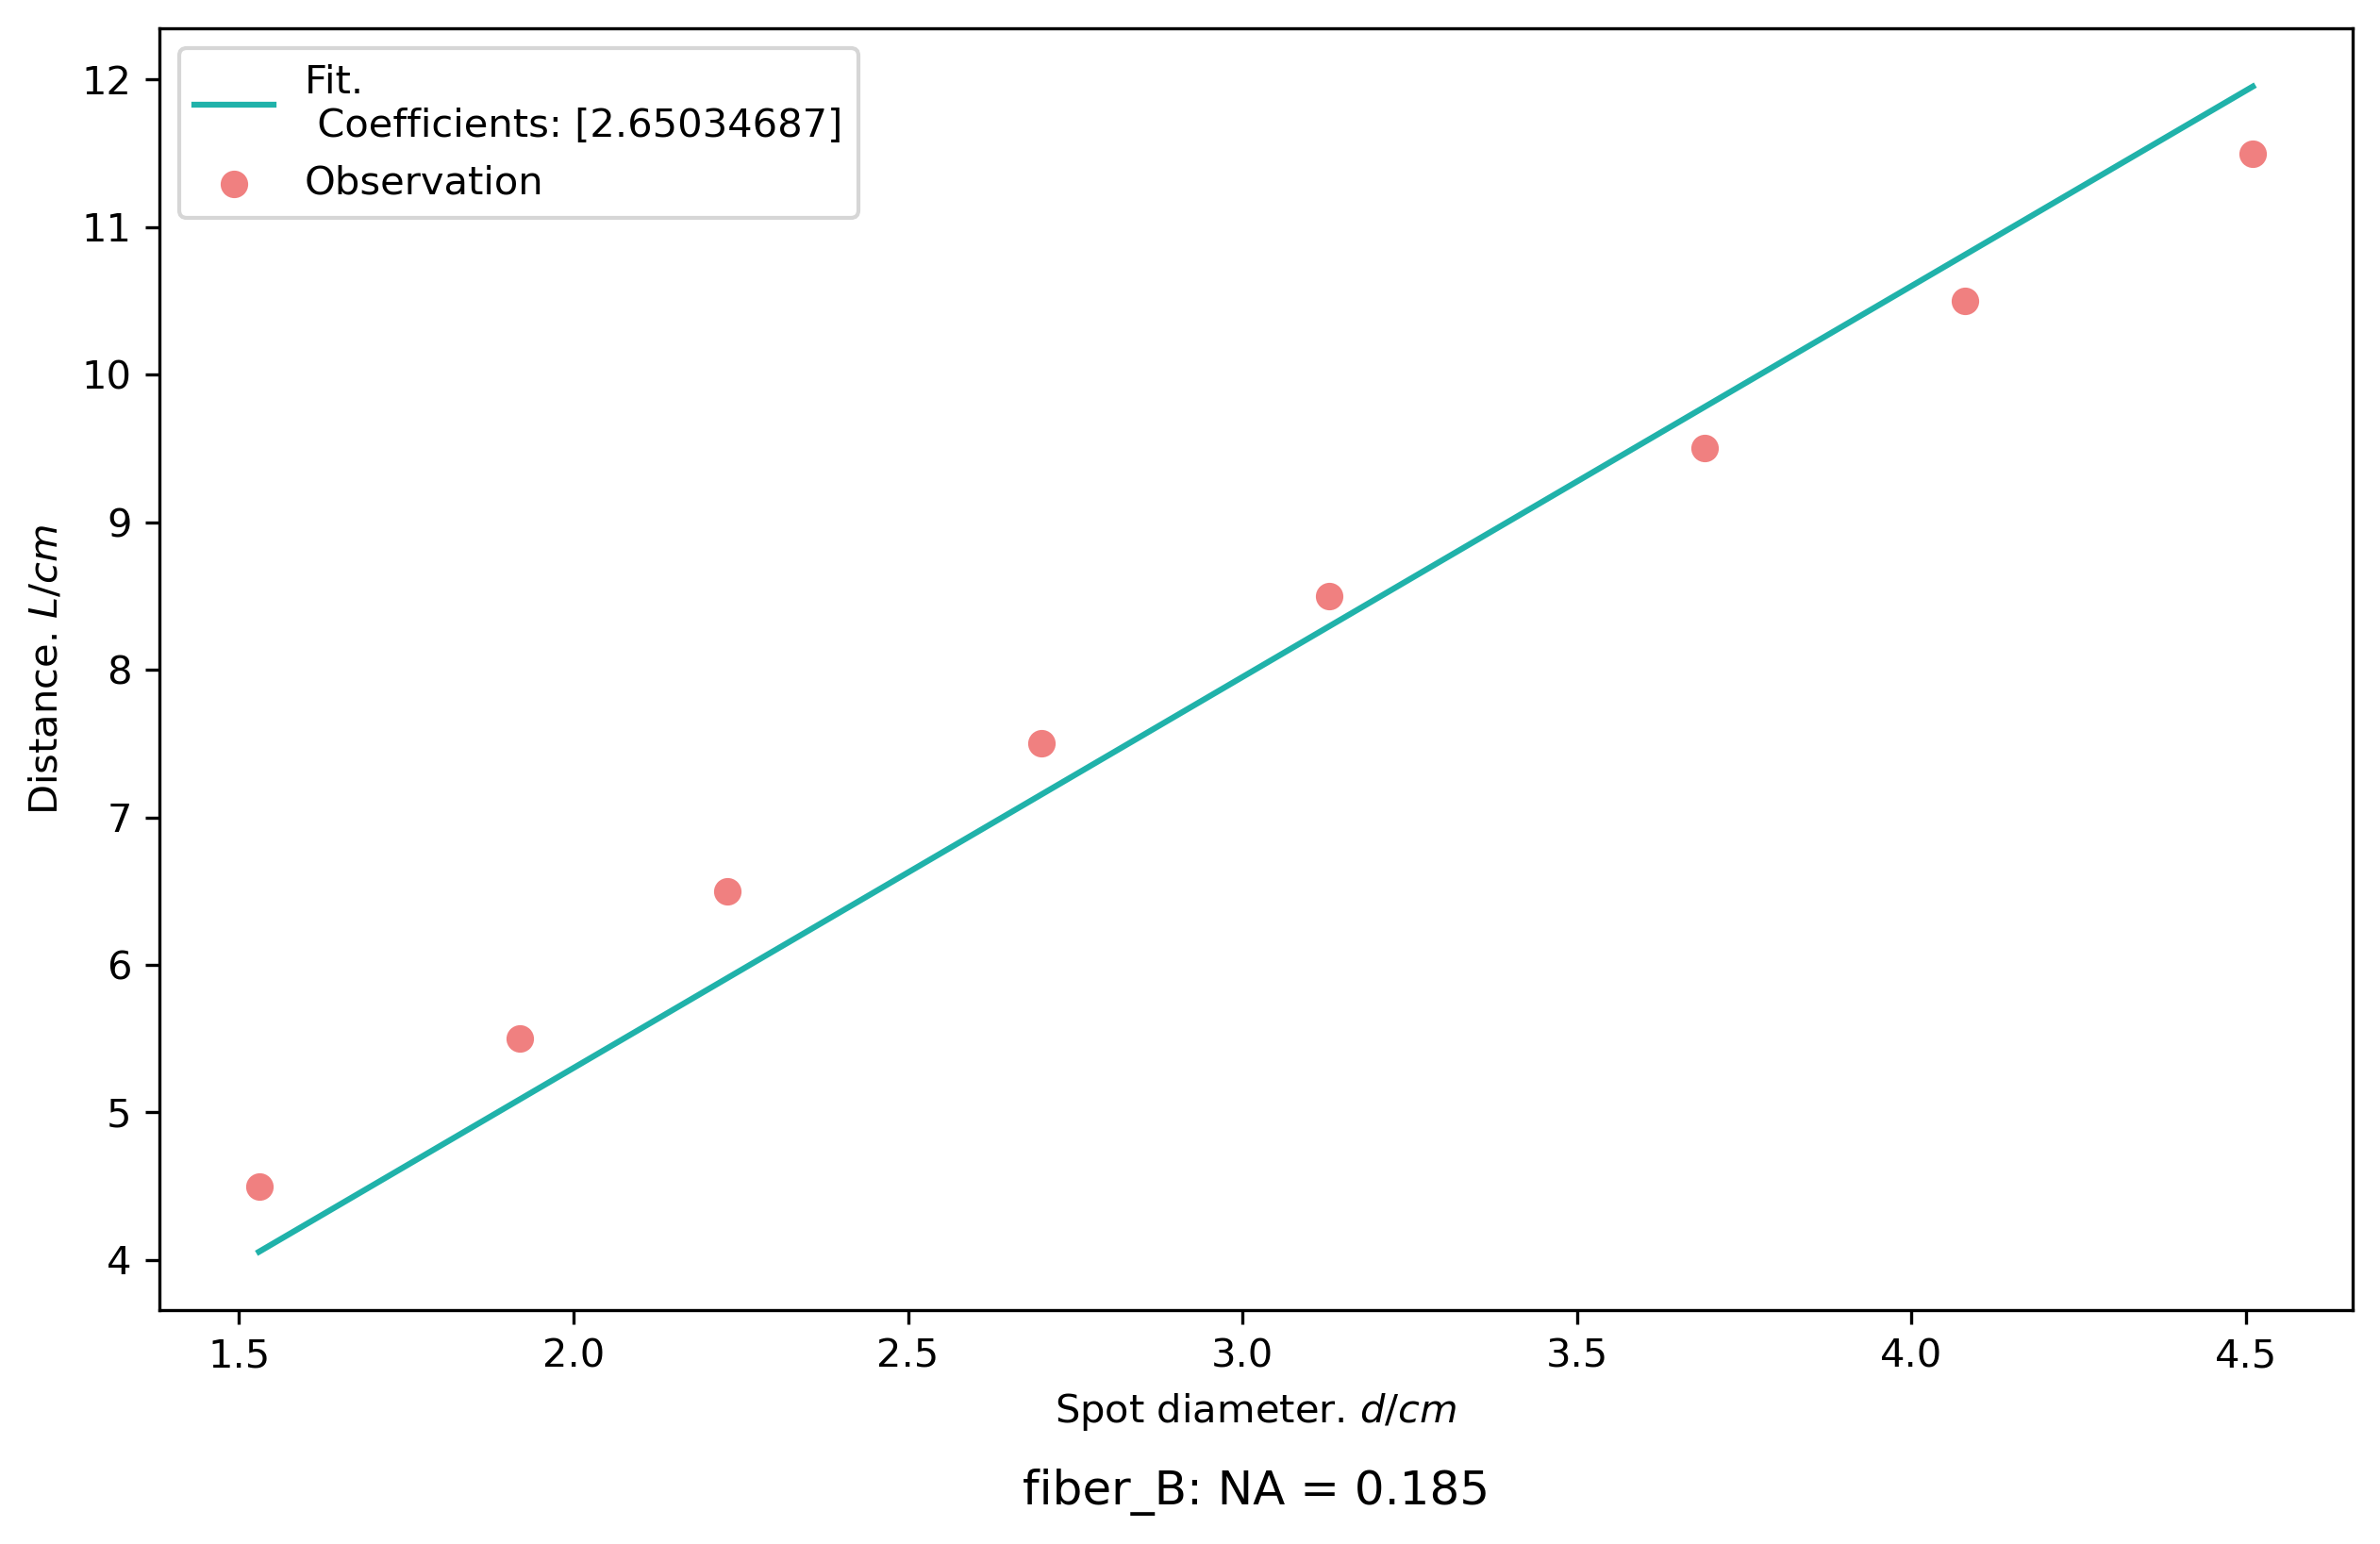
\includegraphics[width=0.3\textwidth]{attachments/fig.1.1.2.png}
		}
		\subfloat[The numerical aperture. $\phi 4\mu m$]{\label{fig.1.1.3}
		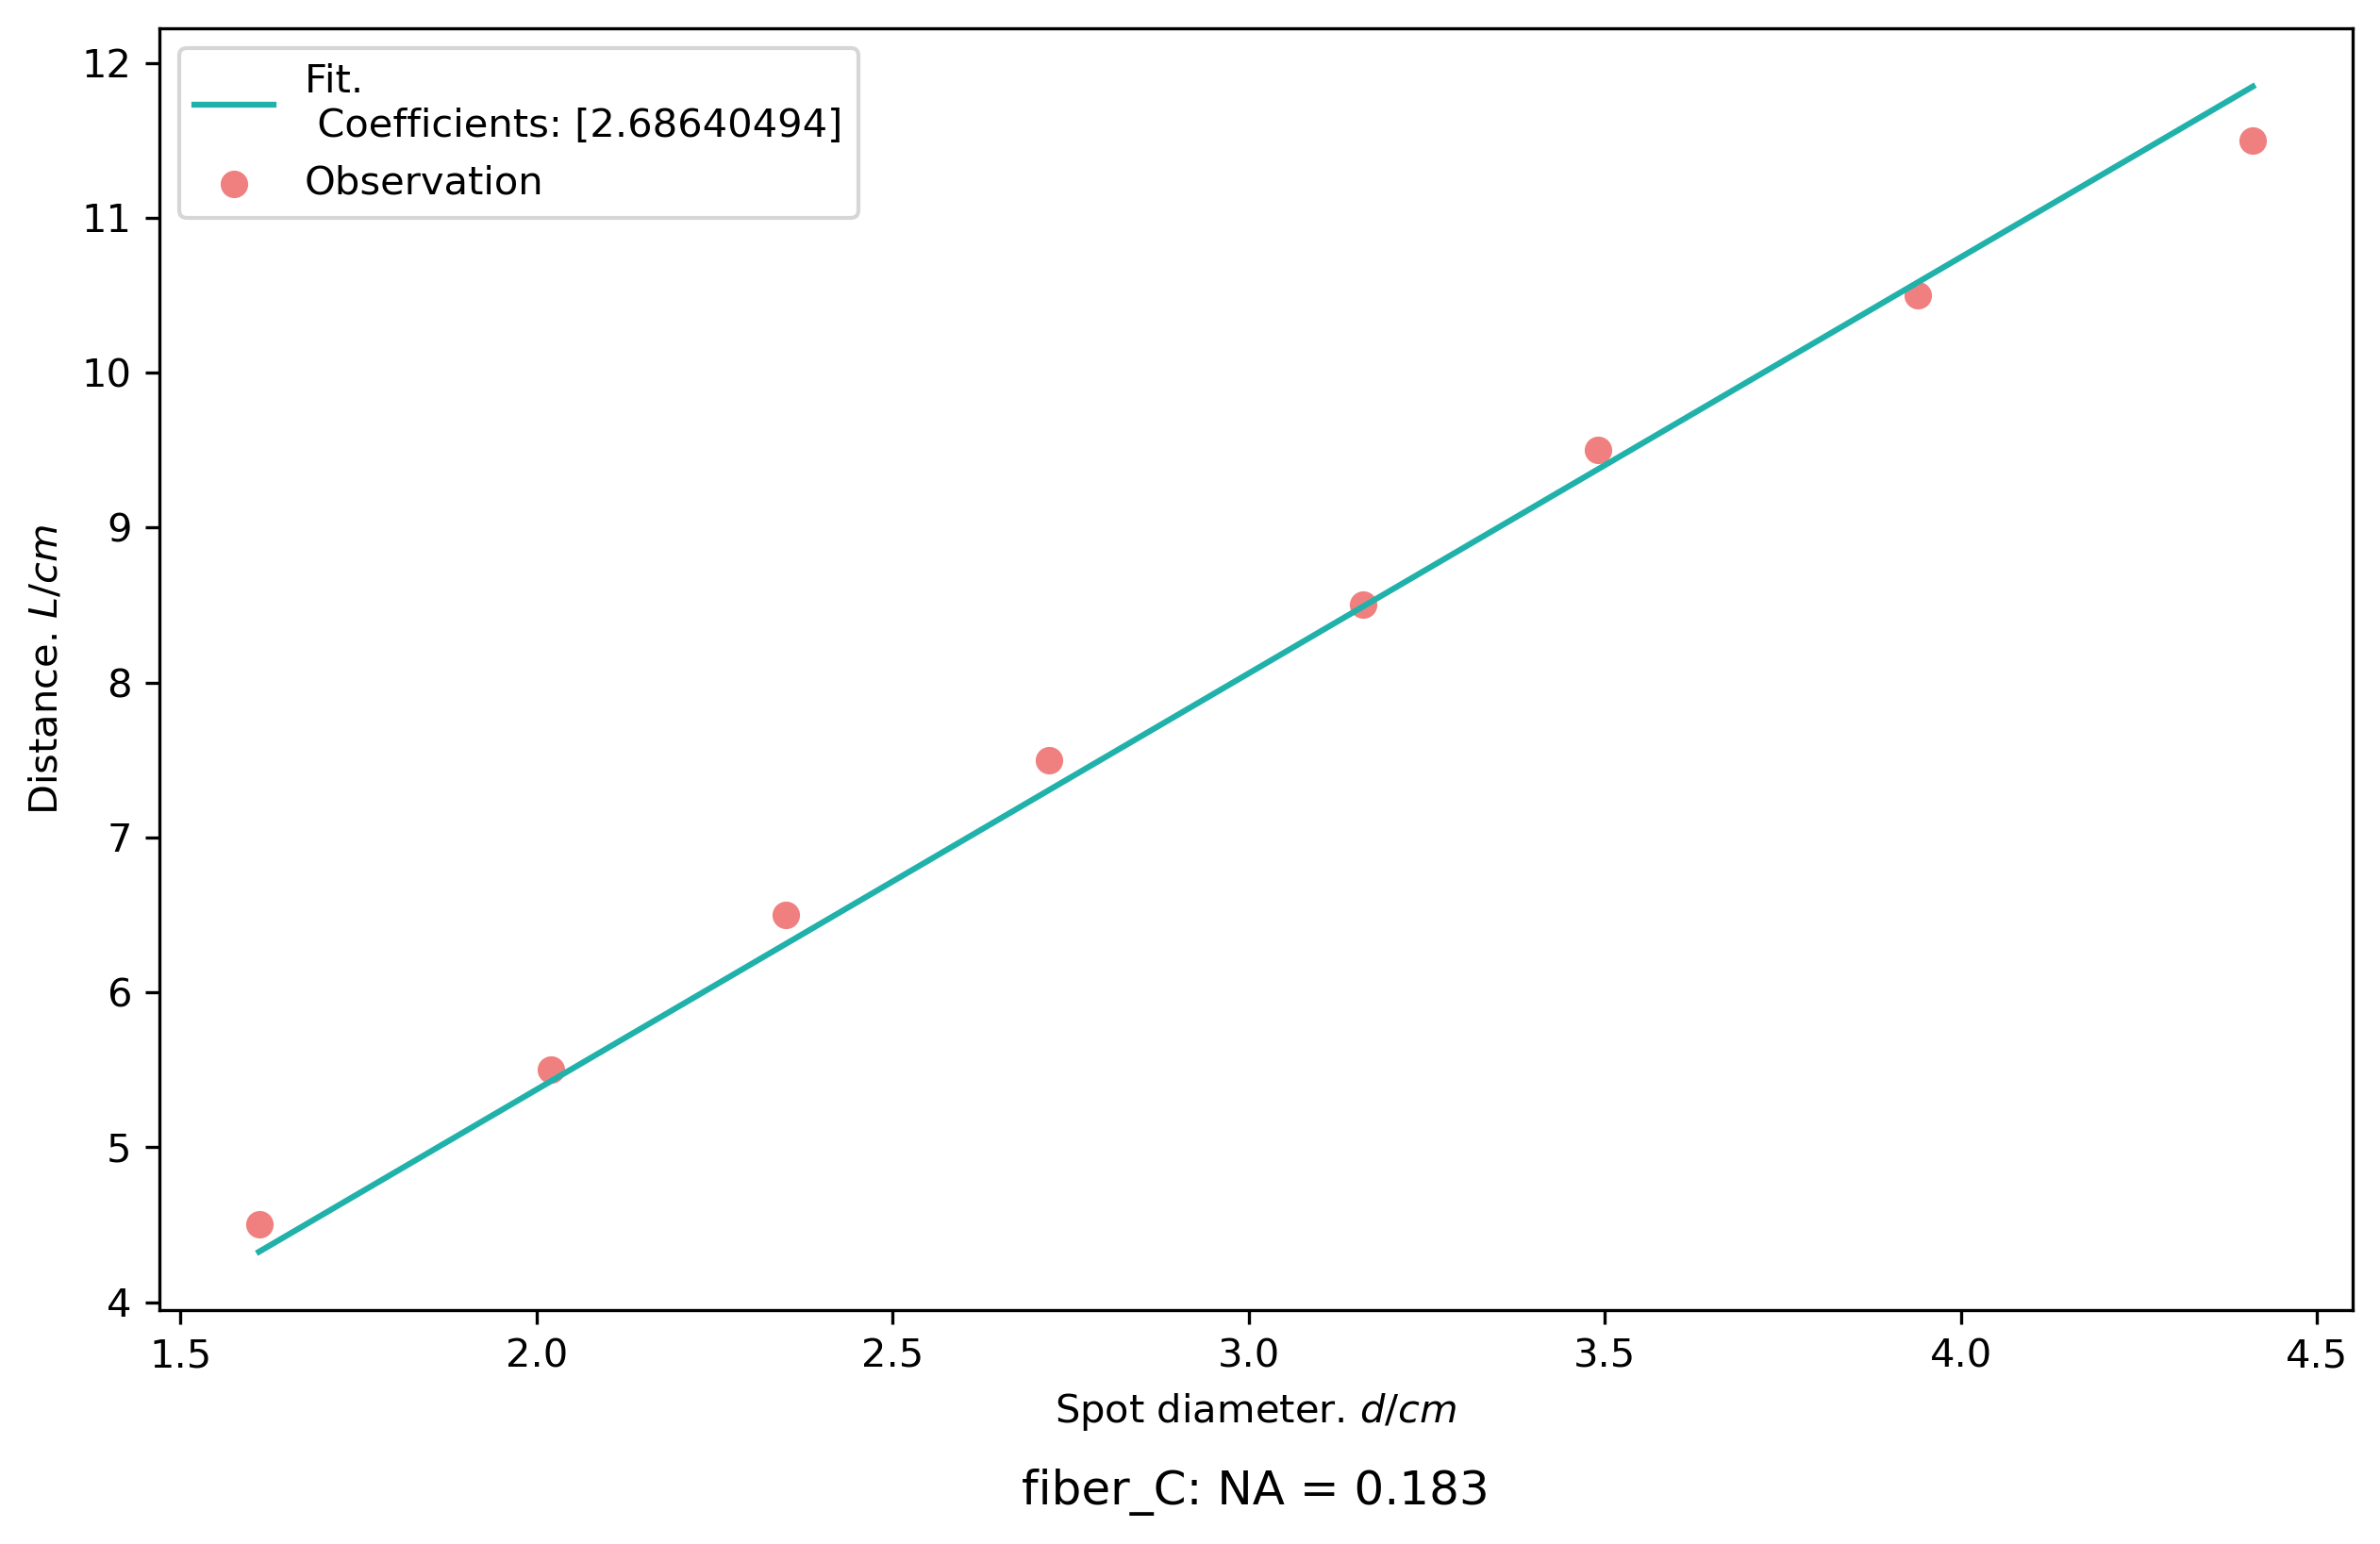
\includegraphics[width=0.3\textwidth]{attachments/fig.1.1.3.png}
		}

		\subfloat[The facula patterns. $\phi 62.5\mu m$]{\label{fig.1.2.1}
		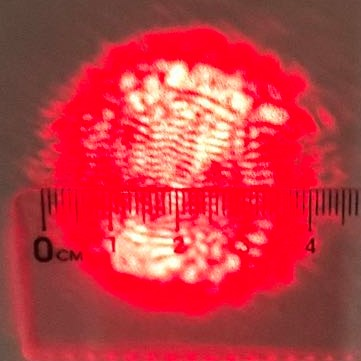
\includegraphics[width=0.3\textwidth]{attachments/fig.1.2.1.jpg}
		}
		\subfloat[The facula patterns. $\phi 9\mu m$]{\label{fig.1.2.2}
		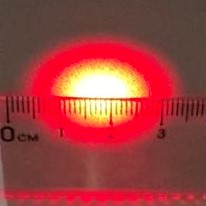
\includegraphics[width=0.3\textwidth]{attachments/fig.1.2.2.jpg}
		}
		\subfloat[The facula patterns. $\phi 4\mu m$]{\label{fig.1.2.3}
		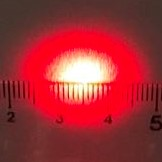
\includegraphics[width=0.3\textwidth]{attachments/fig.1.2.3.jpg}
		}
		\caption{\textbf{The facula patterns and the numerical aperture}}
		\label{fig.1}
	\end{figure*}
	\begin{table*}[htbp]
		\centering
			\begin{tabular}{lc}
				\toprule
				Fiber & Numerical aperture \\
				\midrule
				$\phi 62.5\mu m$ & 0.277 \\
				$\phi 9\mu m$ & 0.185 \\
				$\phi 4\mu m$ & 0.183 \\
				\bottomrule
			\end{tabular}
			\caption{\textbf{The numerical aperture of the three fibers}}
			\label{tab.2.1}
	\end{table*}

	\subsection{Impact of transmission in a fiber on the polarization state}
	We first generated two linearly polarized lights ($L_{+\frac{\pi}{4}}$ and $L_{+\frac{13\pi}{36}}$) and one left-hand circularly polarized lights ($L_R$) and measure their Stokes parameters in the free space.

	\paragraph{A. linearly polarized lights $L_{+\frac{\pi}{4}}$}~
	\newline 
	\indent
	\begin{enumerate}[label=\arabic*.]
		\item Angle: $\phi = \frac{\pi}{4}$, $\chi = 0$
		\item Light power($mW$): $P = (P_x, P_y, P_{+\frac{\pi}{4}}, P_R) = (0.315, 0.305, 0.615, 0.321)$
		\item Experimental Stocks vector: 
		$S=(S_0, S_1, S_2, S_3)^T = (0.620, 0.010, 0.610, -0.022)$
		\item Normalized experimental Stocks vector: $S=(S_0, S_1, S_2, S_3)^T = (1.000, 0.016, 0.984, -0.035)$
		\item Theoretical Stocks vector: $S=(S_0, S_1, S_2, S_3)^T = (0.610, 0.00, 0.610, 0.00)$
		\item Normalized theoretical Stocks vector: $S=(S_0, S_1, S_2, S_3)^T = (1.000, 0.000, 1.000, 0.000)$
	\end{enumerate}

	\paragraph{B. linearly polarized lights $L_{+\frac{13\pi}{36}}$}~
	\newline 
	\indent
	\begin{enumerate}[label=\arabic*.]
		\item Angle: $\phi = \frac{13\pi}{36}$, $\chi = 0$
		\item Light power($mW$): $P = (P_x, P_y, P_{+\frac{\pi}{4}}, P_R) = (0.105, 0.508, 0.535, 0.290)$
		\item Experimental Stocks vector: $S=(S_0, S_1, S_2, S_3)^T = (0.613, -0.403, 0.457, 0.033)$
		\item Normalized experimental Stocks vector: $S=(S_0, S_1, S_2, S_3)^T = (1.000, -0.657, 0.746, 0.054)$
		\item Theoretical Stocks vector: $S=(S_0, S_1, S_2, S_3)^T = (0.610, -0.392, 0.467, 0.000)$
		\item Normalized theoretical Stocks vector: $S=(S_0, S_1, S_2, S_3)^T = (1.000, -0.643, 0.766, 0.000)$
	\end{enumerate}

	\paragraph{C. left-hand circularly polarized lights $L_R$}~
	\newline 
	\indent
	\begin{enumerate}[label=\arabic*.]
		\item Angle: $\phi = 0$, $\chi = -\frac{\pi}{4}$
		\item Light power($mW$): $P = (P_x, P_y, P_{+\frac{\pi}{4}}, P_R) = (0.307, 0.294, 0.312, 0.602)$
		\item Experimental Stocks vector: $S=(S_0, S_1, S_2, S_3)^T = (0.601, 0.013, 0.023, -0.603)$
		\item Normalized experimental Stocks vector: $S=(S_0, S_1, S_2, S_3)^T = (1.00, 0.022, 0.038, -1.003)$
		\item Theoretical Stocks vector: $S=(S_0, S_1, S_2, S_3)^T = (0.604, 0.000, 0.000, 0.604)$
		\item Normalized theoretical Stocks vector: $S=(S_0, S_1, S_2, S_3)^T = (1.000, 0.000, 0.000, -1.000)$
	\end{enumerate}

	We found our measurements accurately conformed to theoretical predictions, which proved that the Stocks parameters are effective representation of the polarization state.
	
	However, unfortunately, when we tried to measure the Stocks parameters of the polarized light after transmission through a fiber, 
	we found that the light power fluctuated in such a great range that it is technically impossible to achieve an accurate reading.
	Thus, we cannot yet provide an unambiguous experimental result.

	The fluctuation of the light power was recorded and provided in the Supplementary Information.

	\subsection{Strain and temperature sensor based on optical-fiber-based Mach-Zehnder interferometer}
	The count of shift of the interference fringes responding to the change of strain and temperature are shown in Fig. \ref{fig.2.1} and Fig. \ref{fig.2.2}, respectively.
	
		\begin{figure*}[htbp]
		\centering
		\subfloat[1st Strain decrease]{\label{fig.2.1.1.1}
		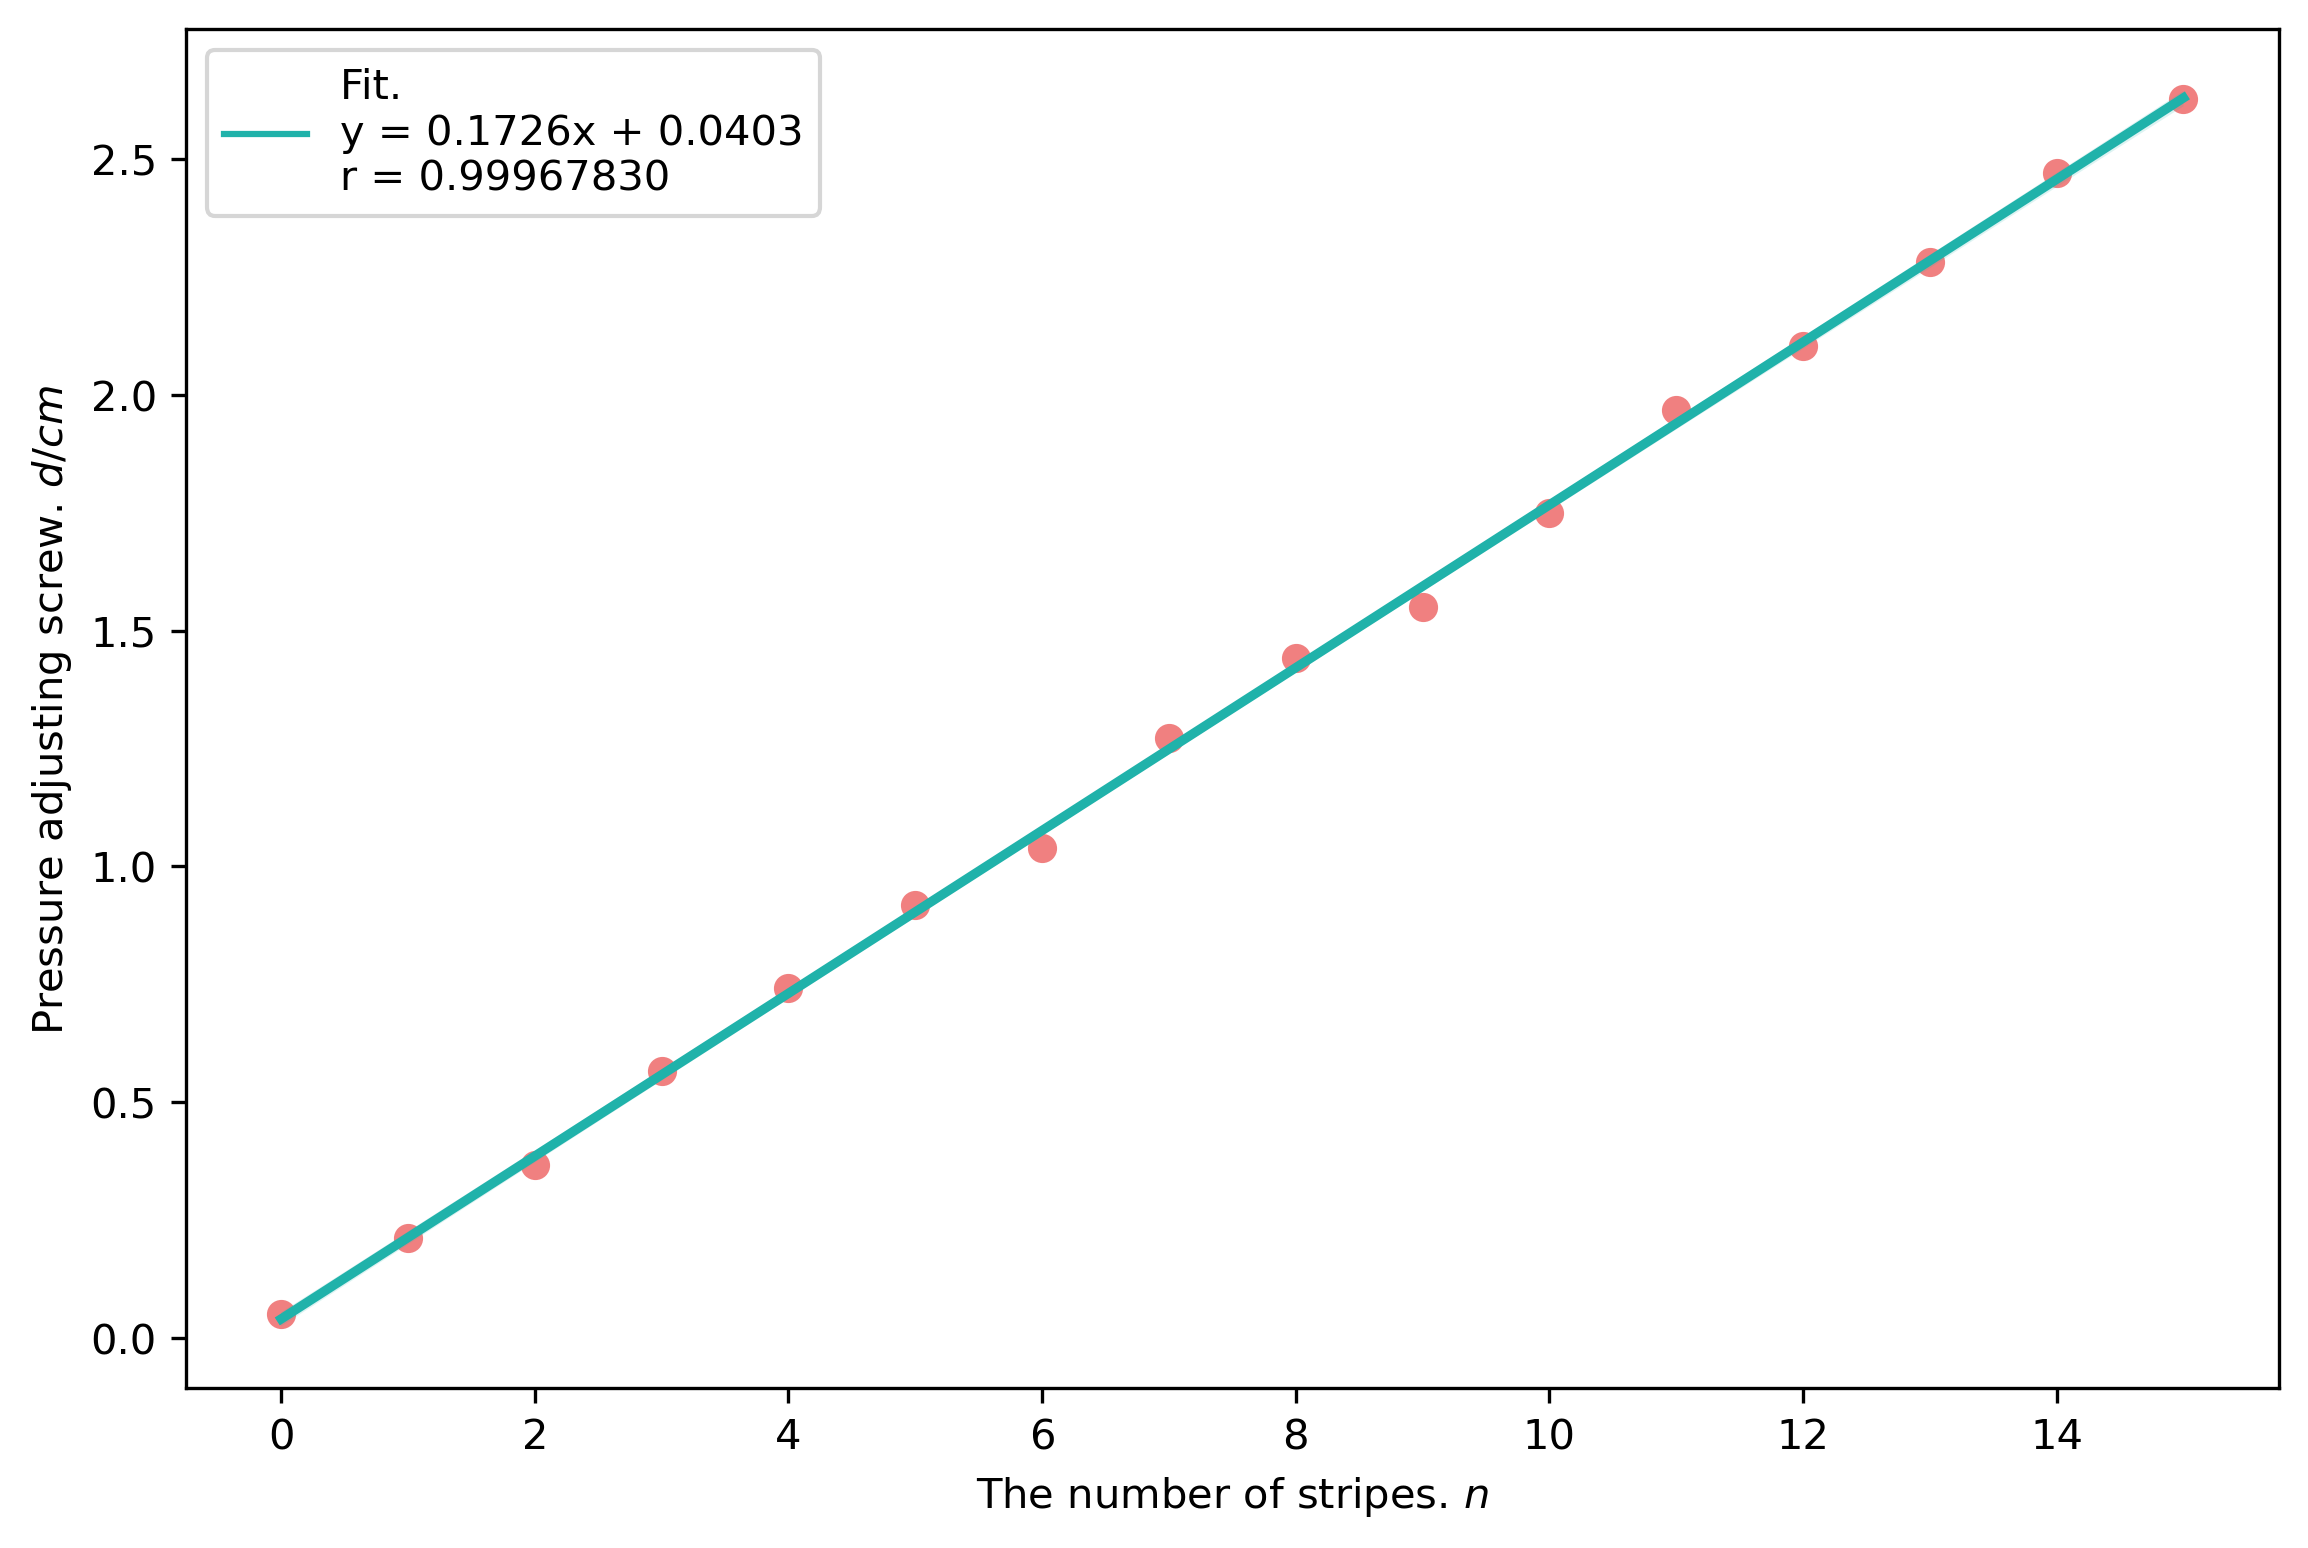
\includegraphics[width=0.4\textwidth]{attachments/fig.2.1.1.1.png}
		}
		\subfloat[1st Strain increase]{\label{fig.2.1.1.2}
		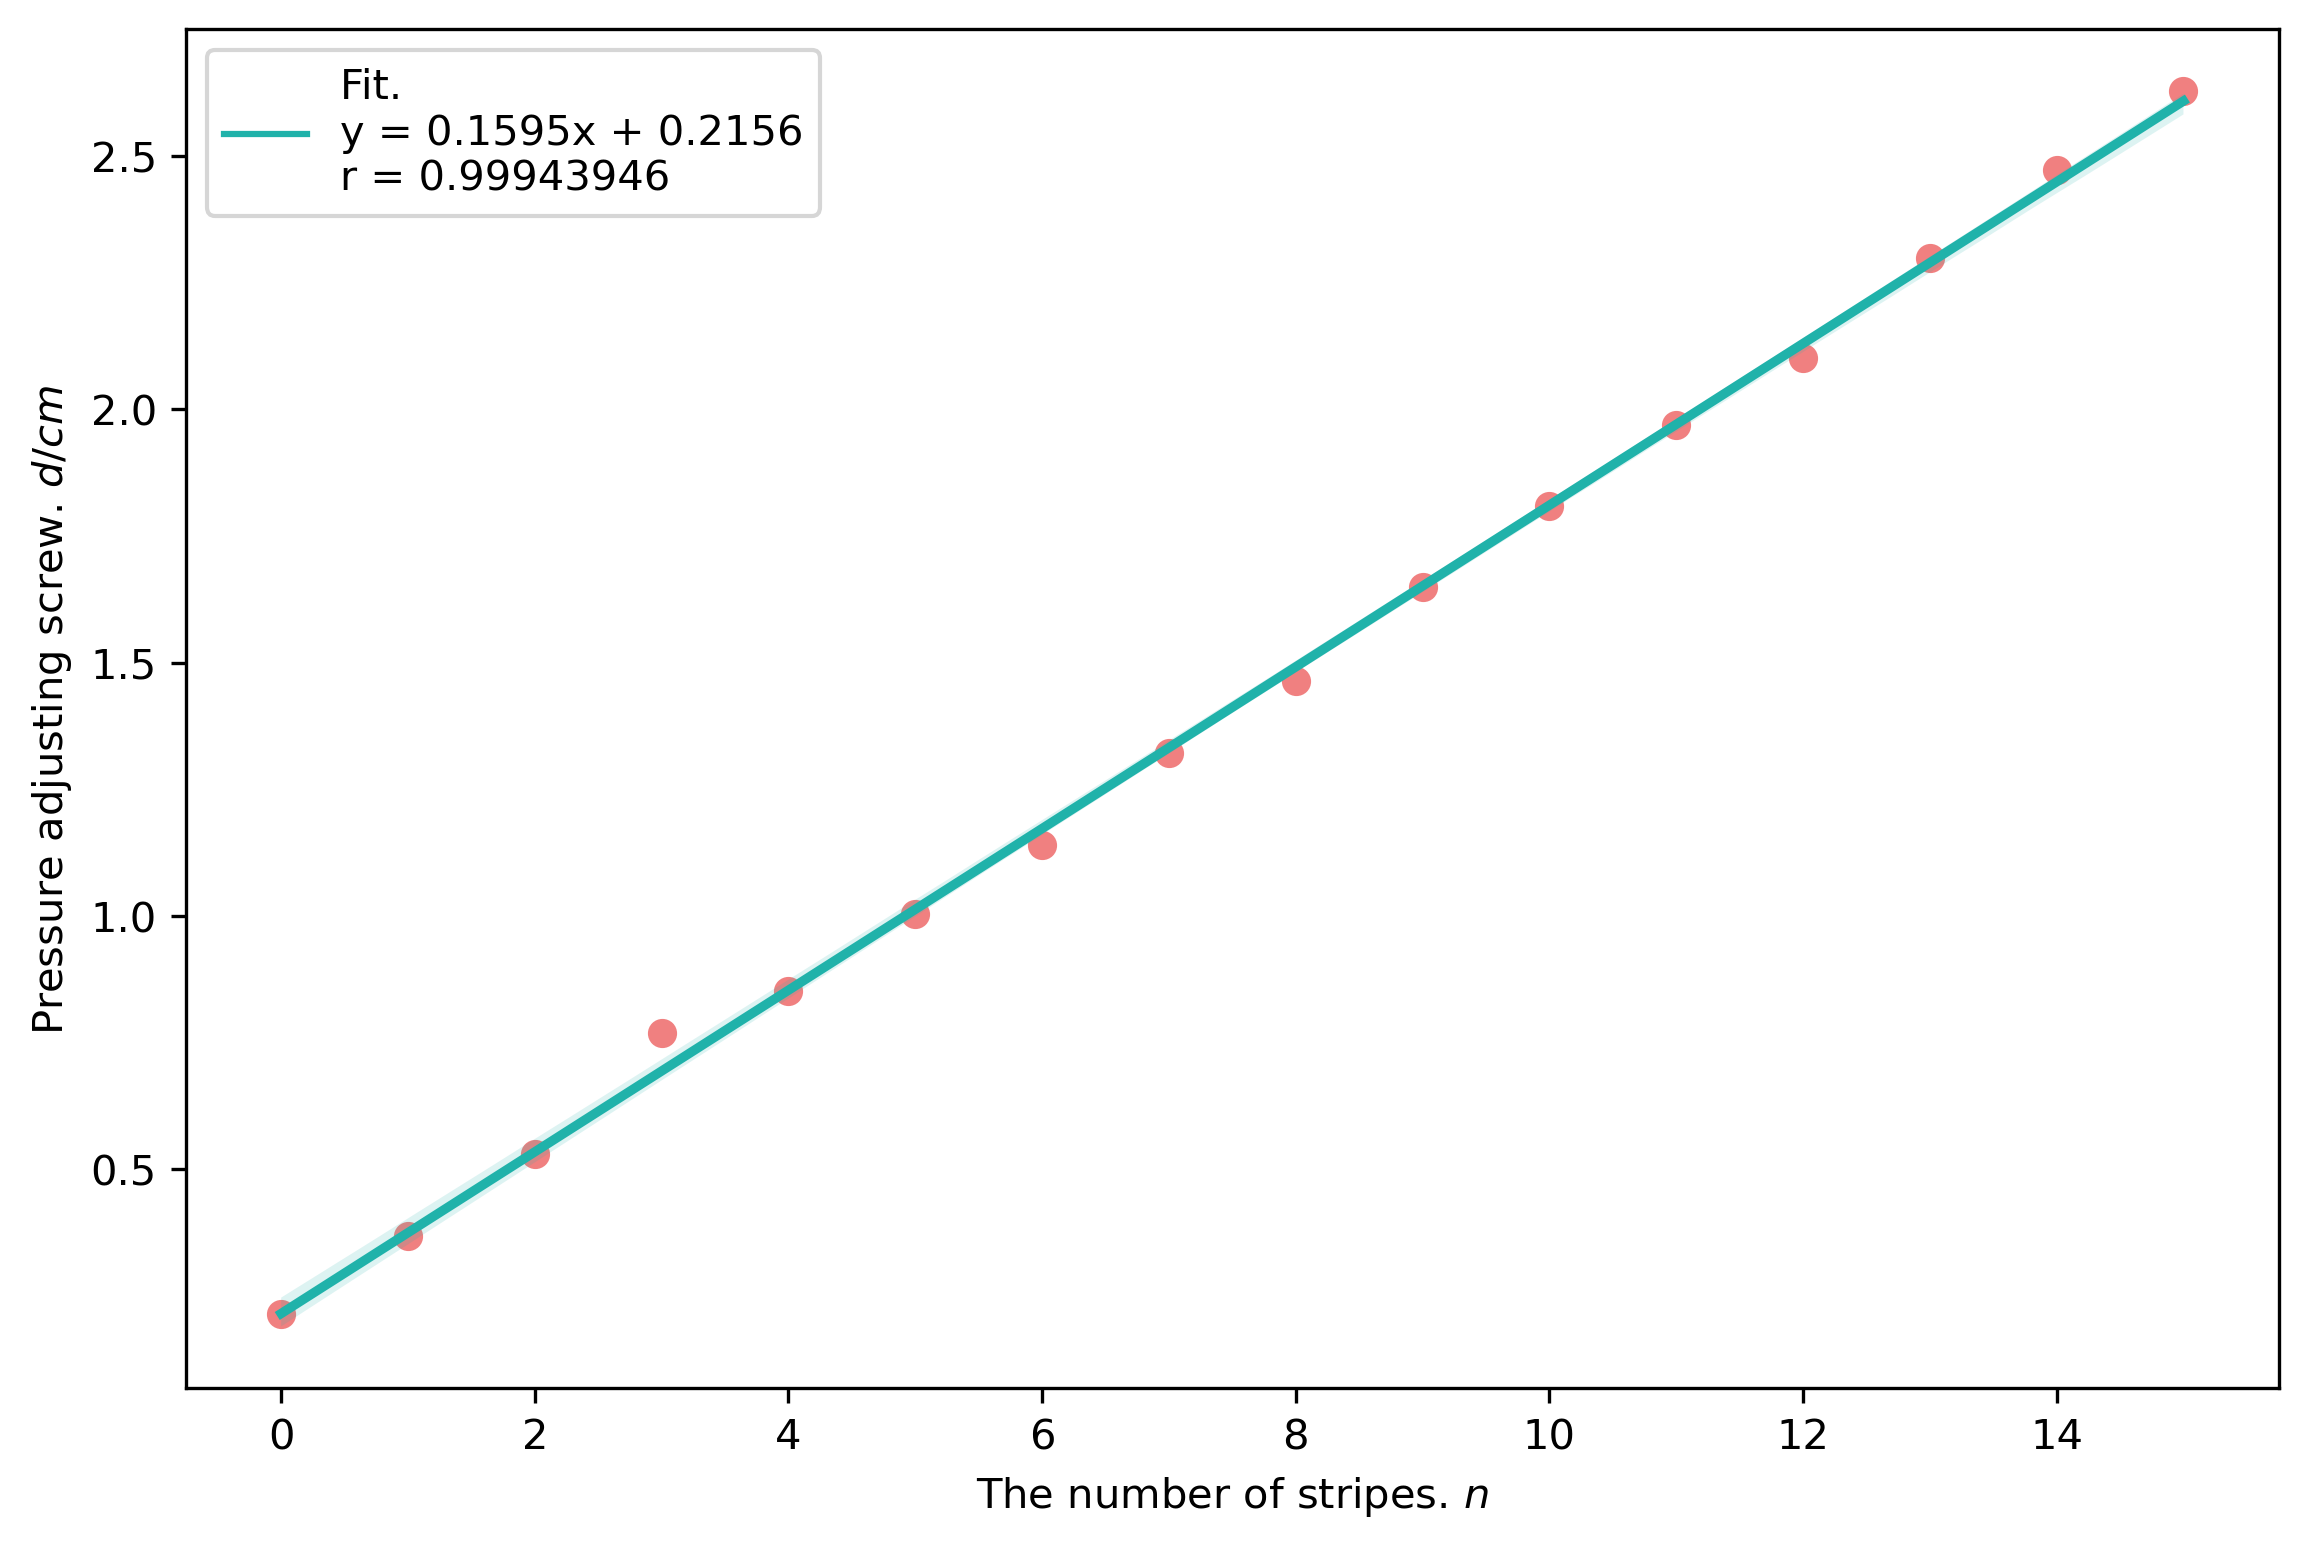
\includegraphics[width=0.4\textwidth]{attachments/fig.2.1.1.2.png}
		}

		\subfloat[2nd Strain decrease]{\label{fig.2.1.2.1}
		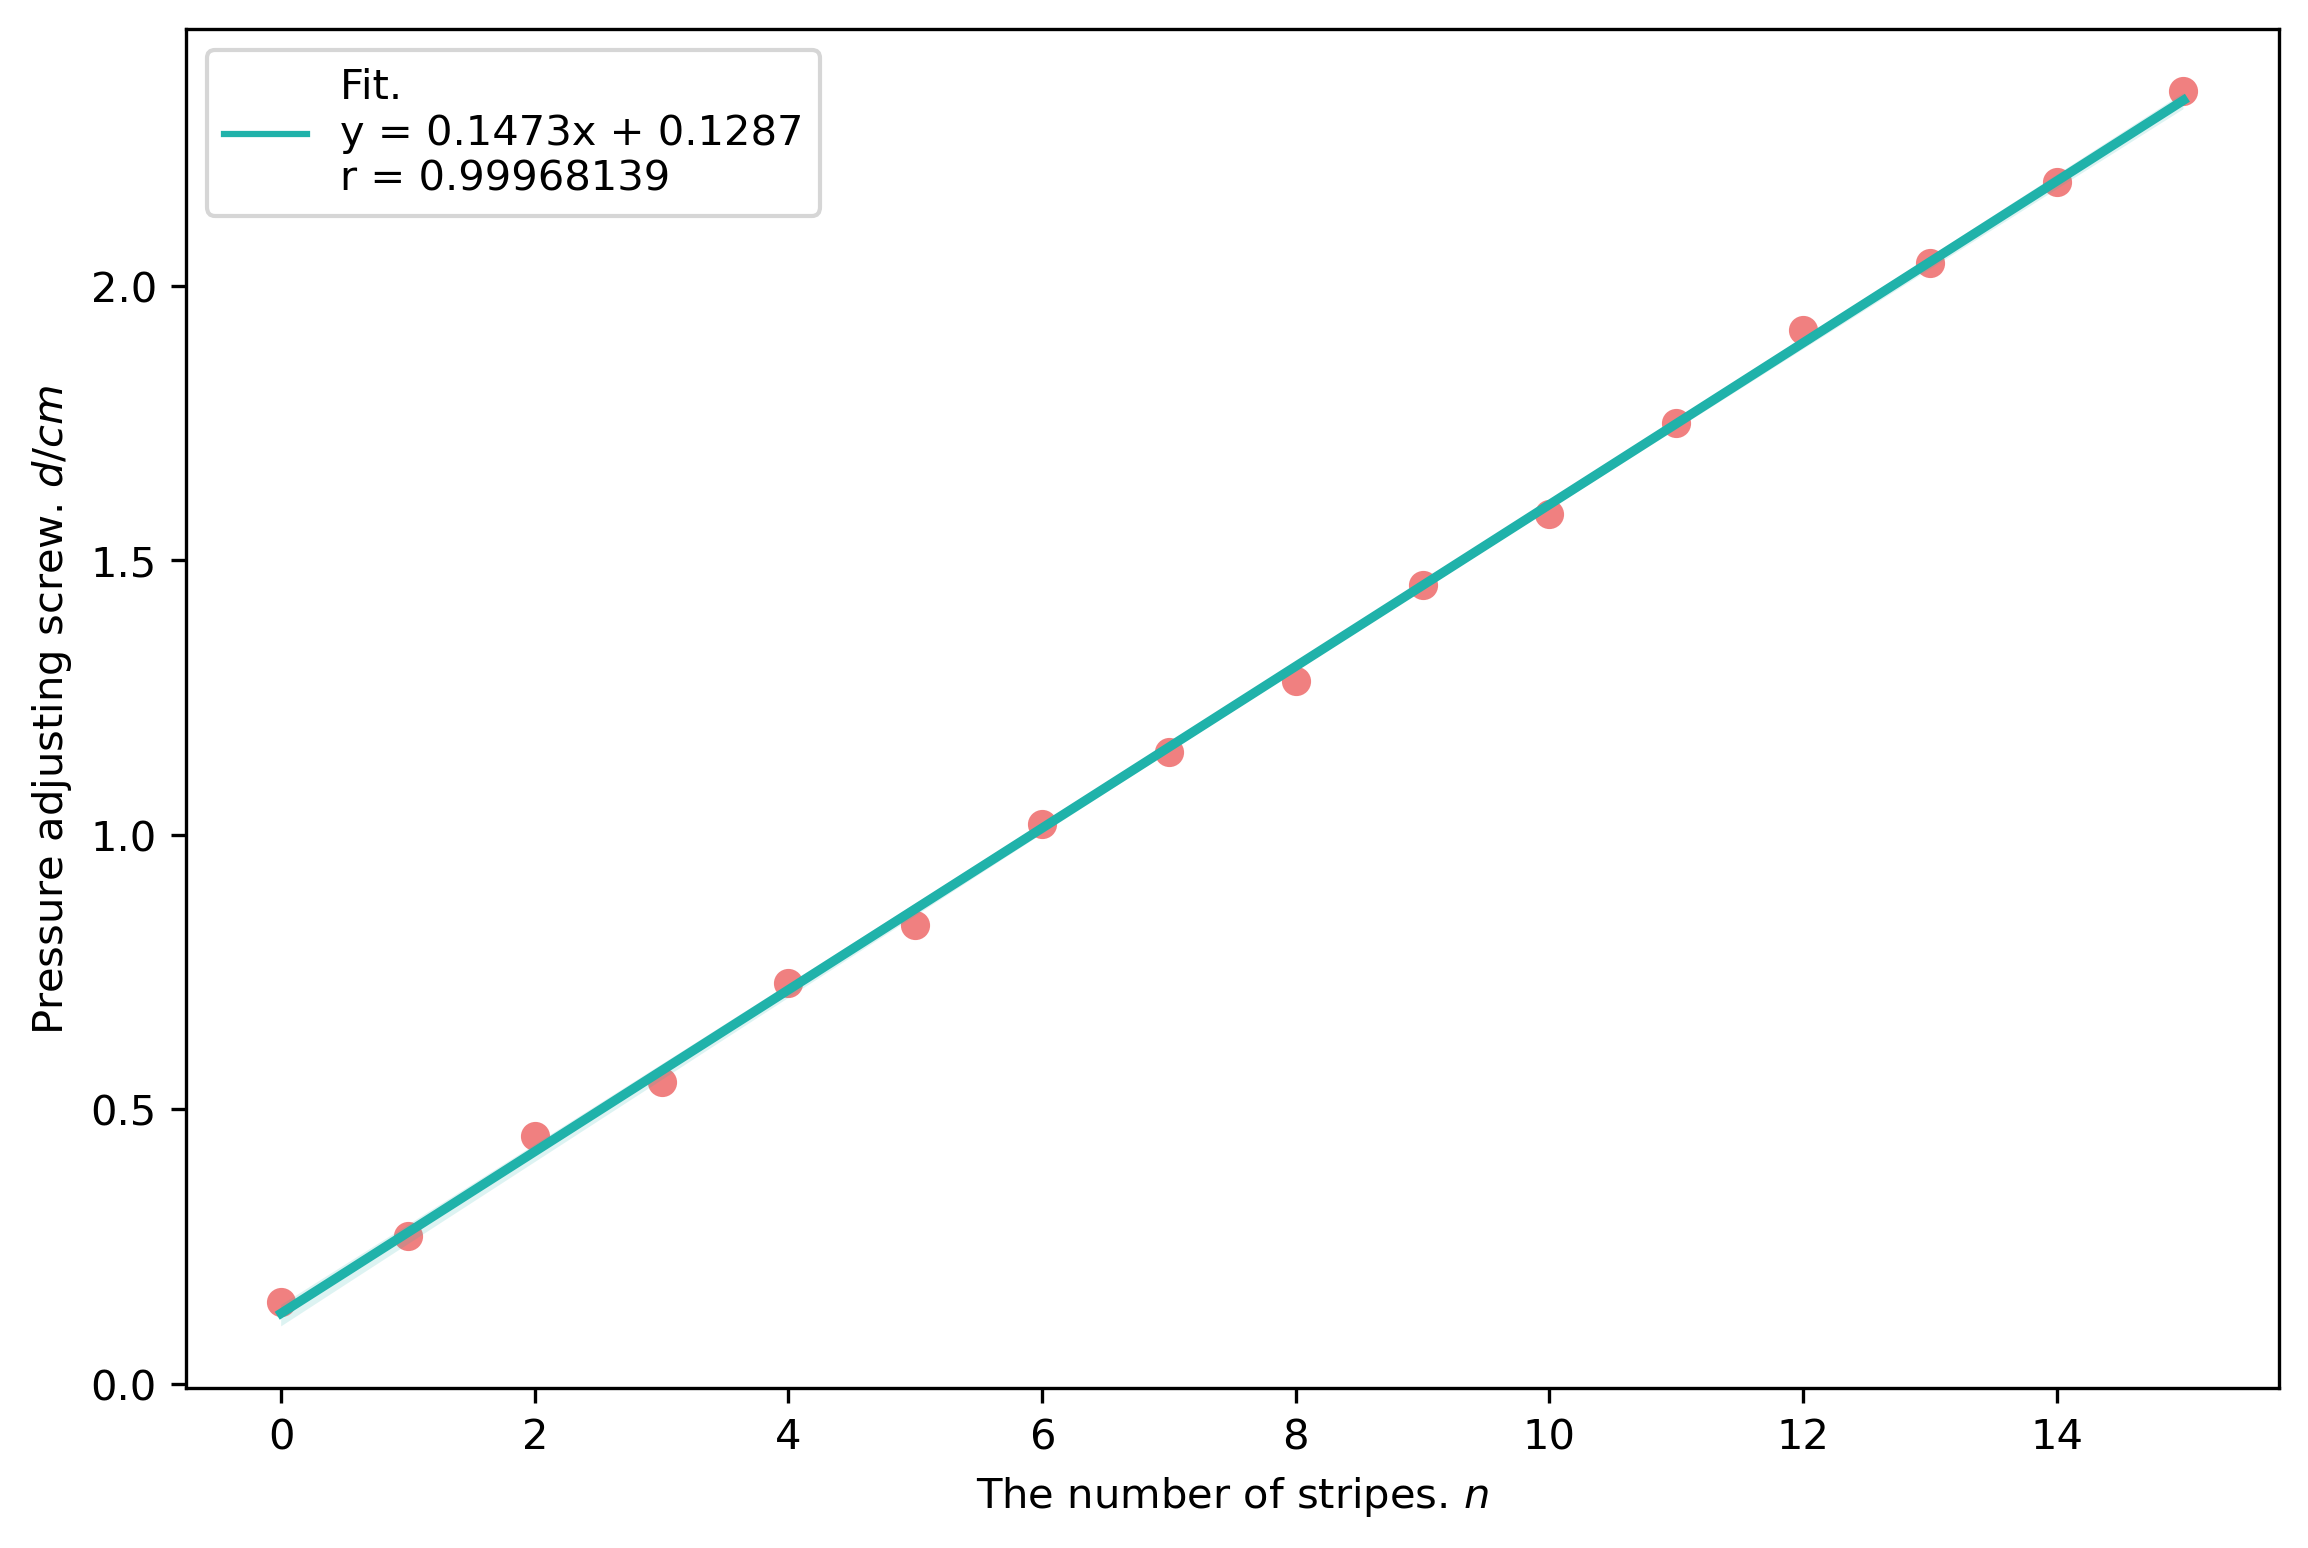
\includegraphics[width=0.4\textwidth]{attachments/fig.2.1.2.1.png}
		}
		\subfloat[2nd Strain increase]{\label{fig.2.1.2.2}
		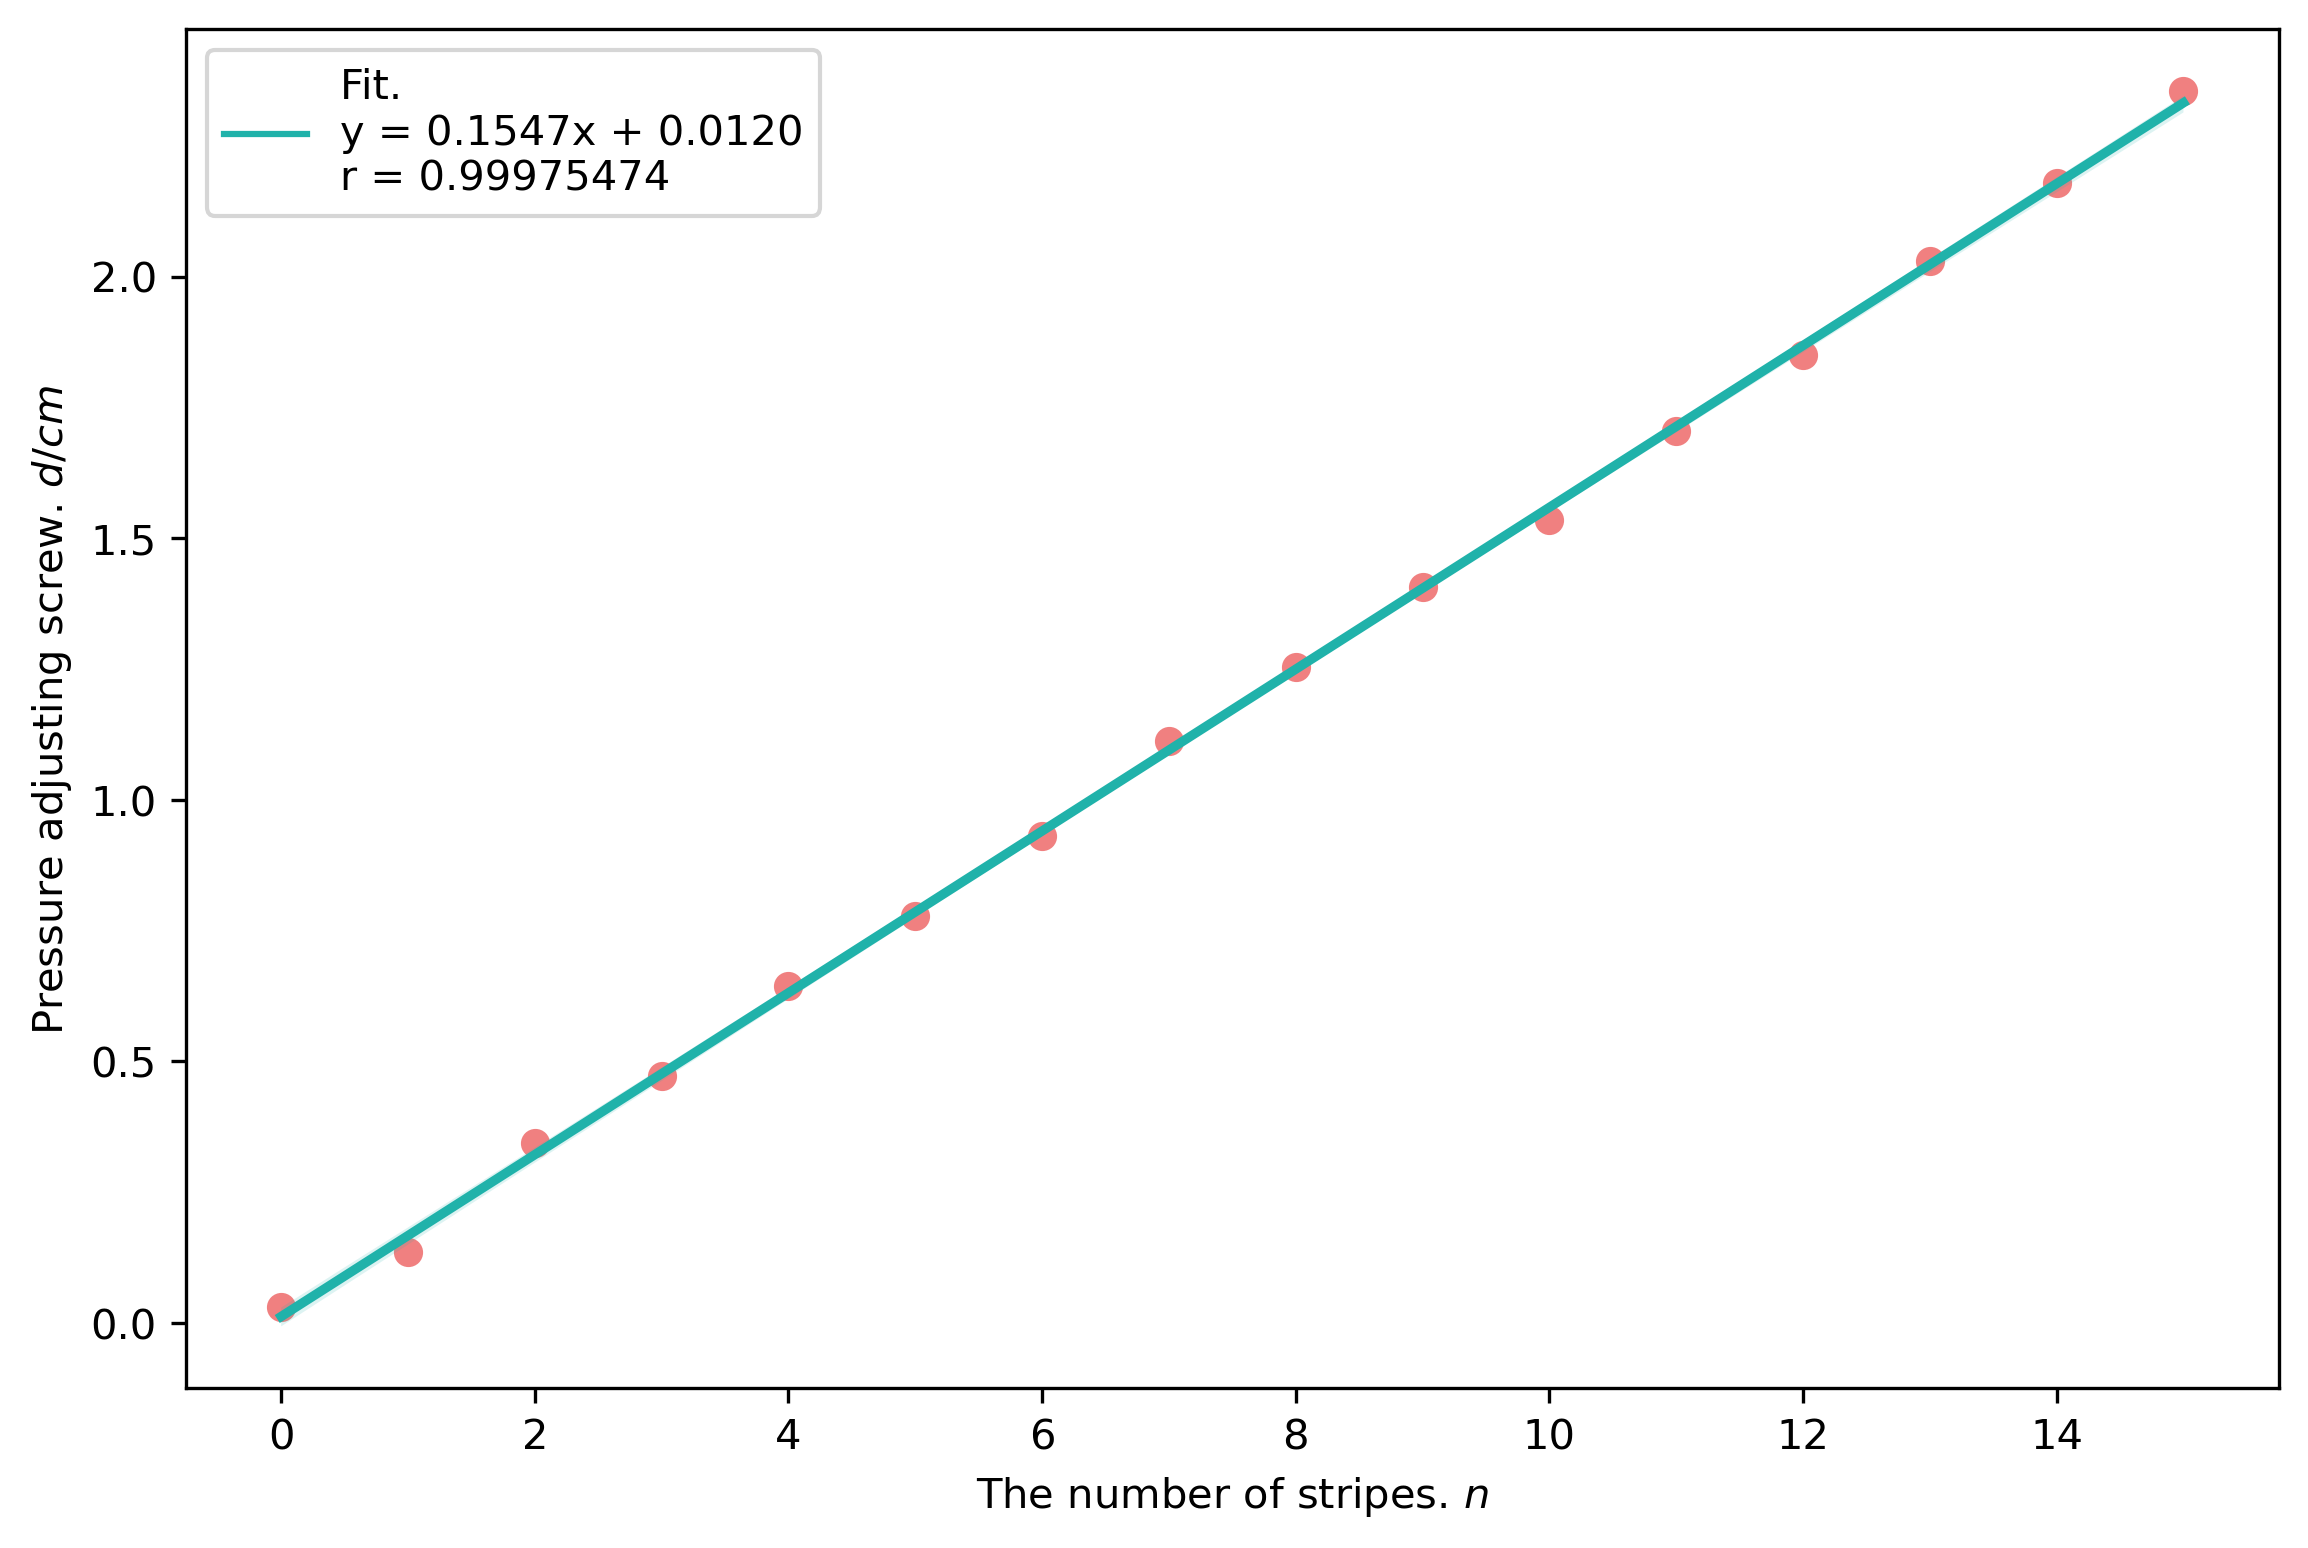
\includegraphics[width=0.4\textwidth]{attachments/fig.2.1.2.2.png}
		}
		\caption{\textbf{Strain sensor}}
		\label{fig.2.1}
	\end{figure*}

	\begin{figure*}[htbp]
		\centering
		\subfloat[1st Temperature decrease]{\label{fig.2.2.1.1}
		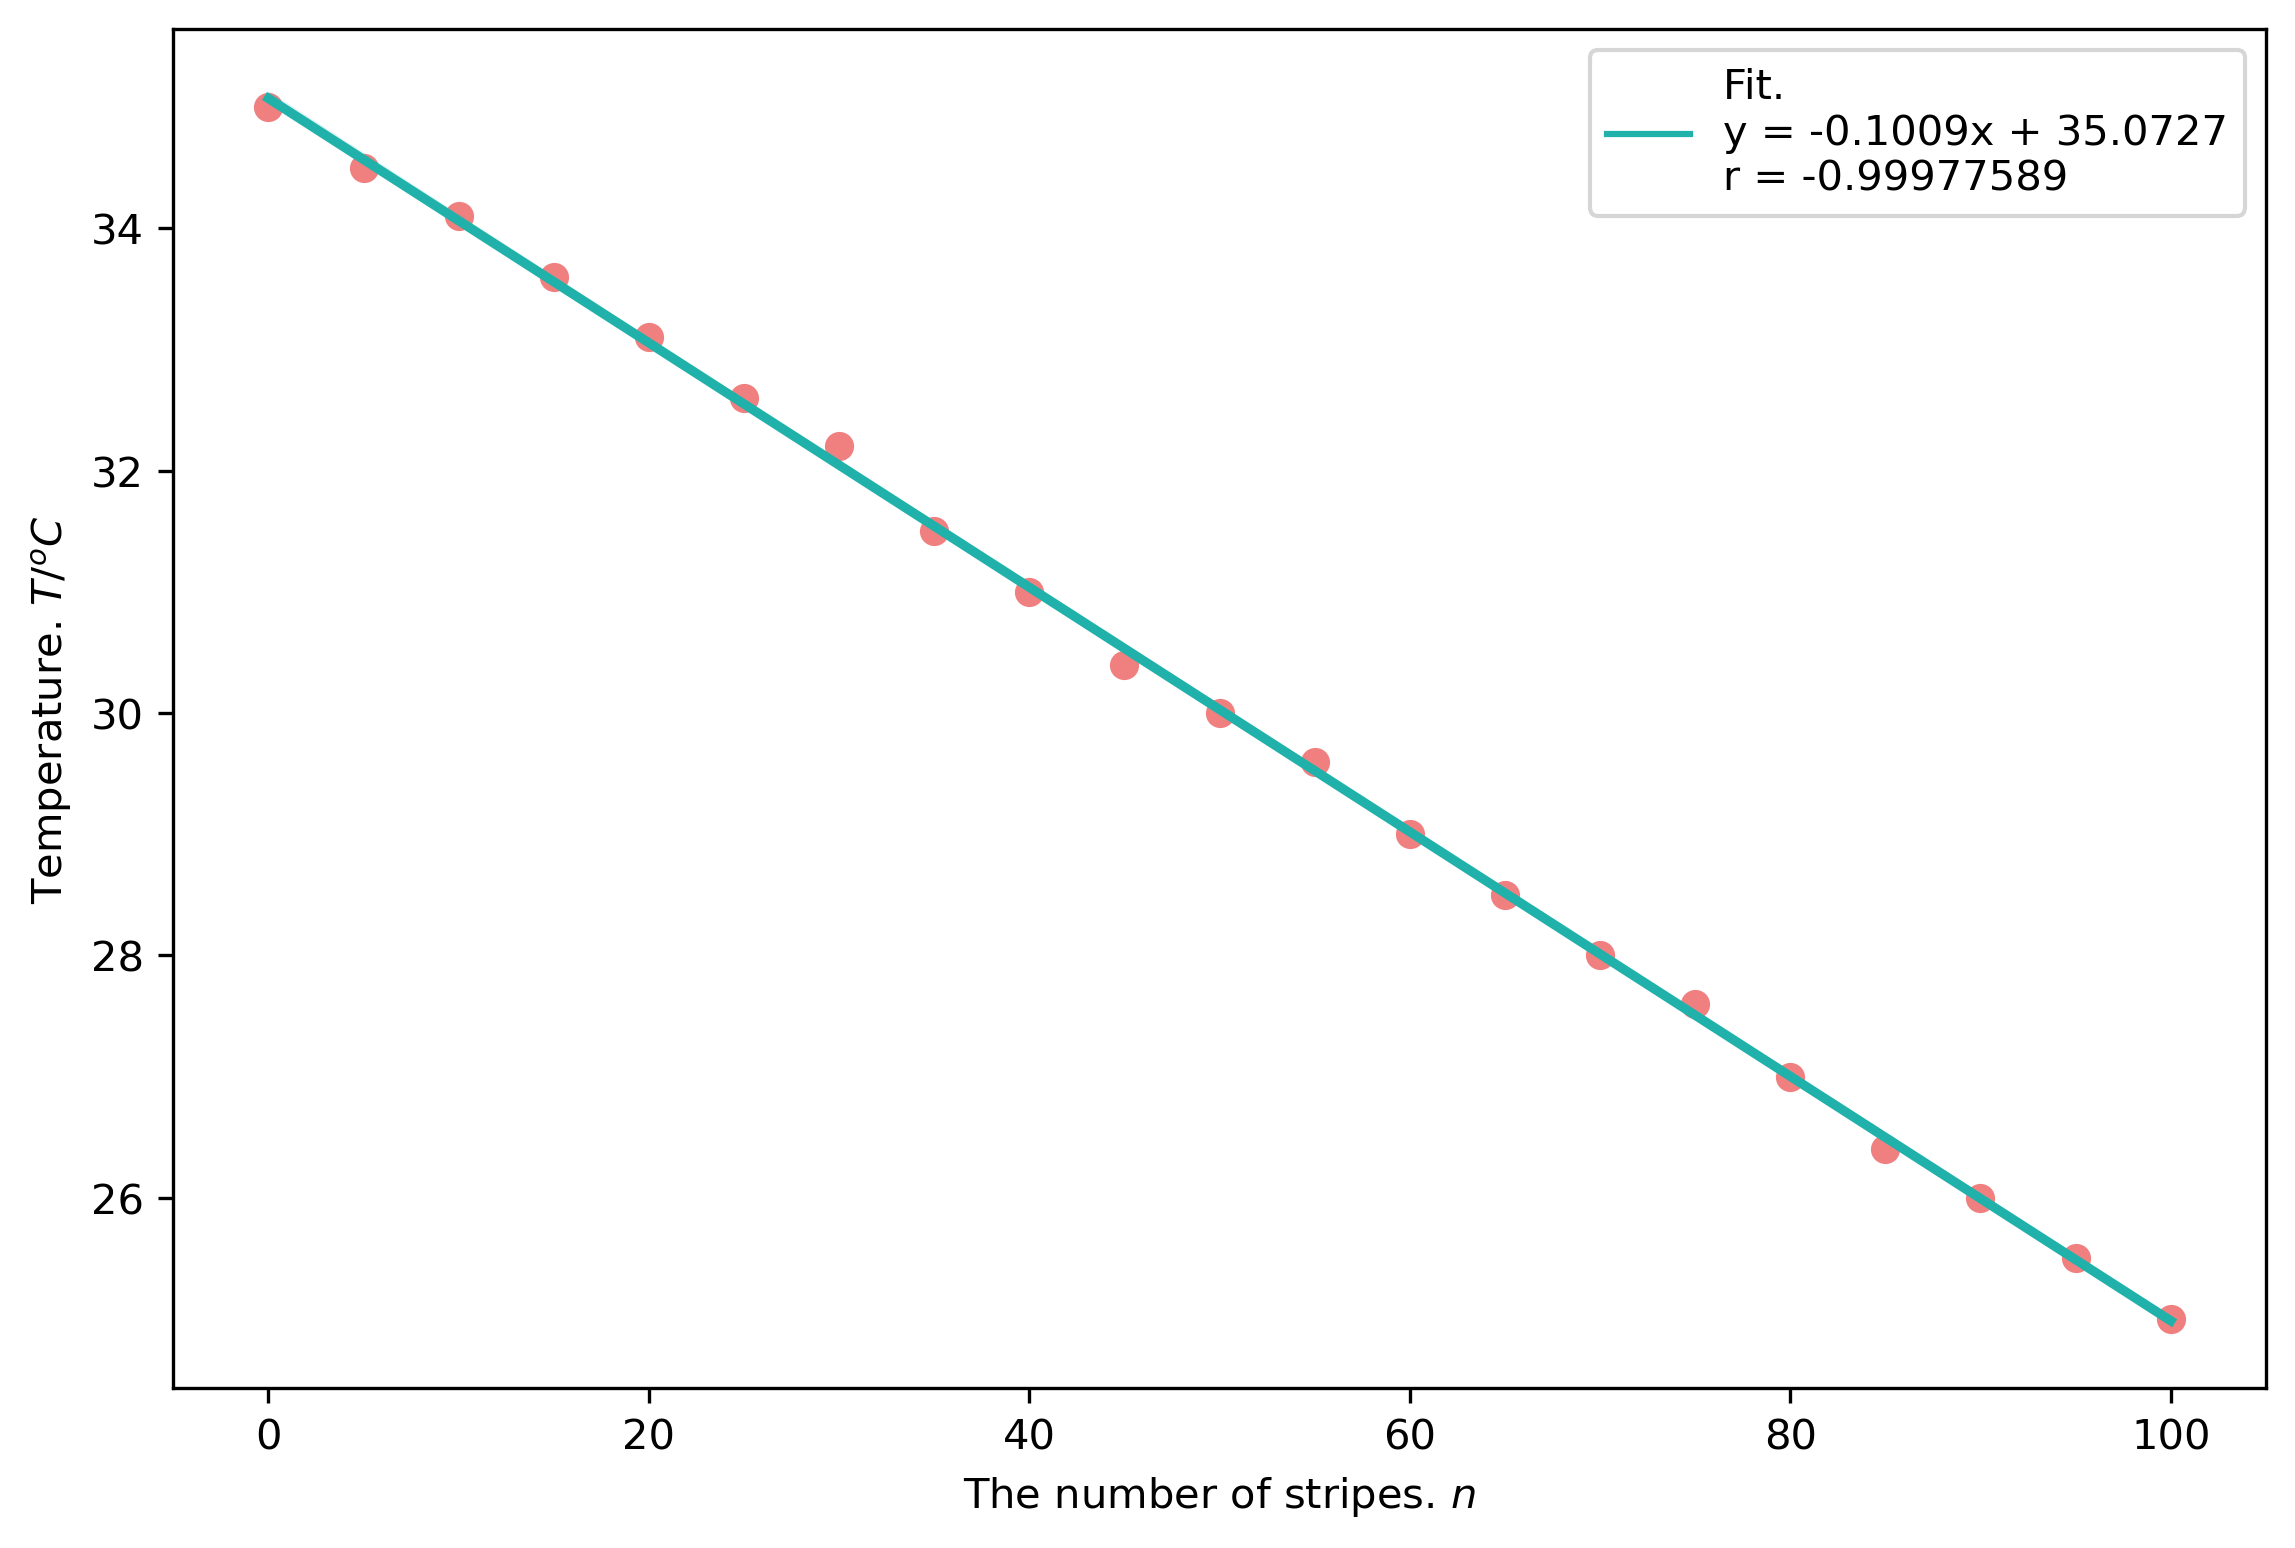
\includegraphics[width=0.4\textwidth]{attachments/fig.2.2.1.1.png}
		}
		\subfloat[1st Temperature increase]{\label{fig.2.2.1.2}
		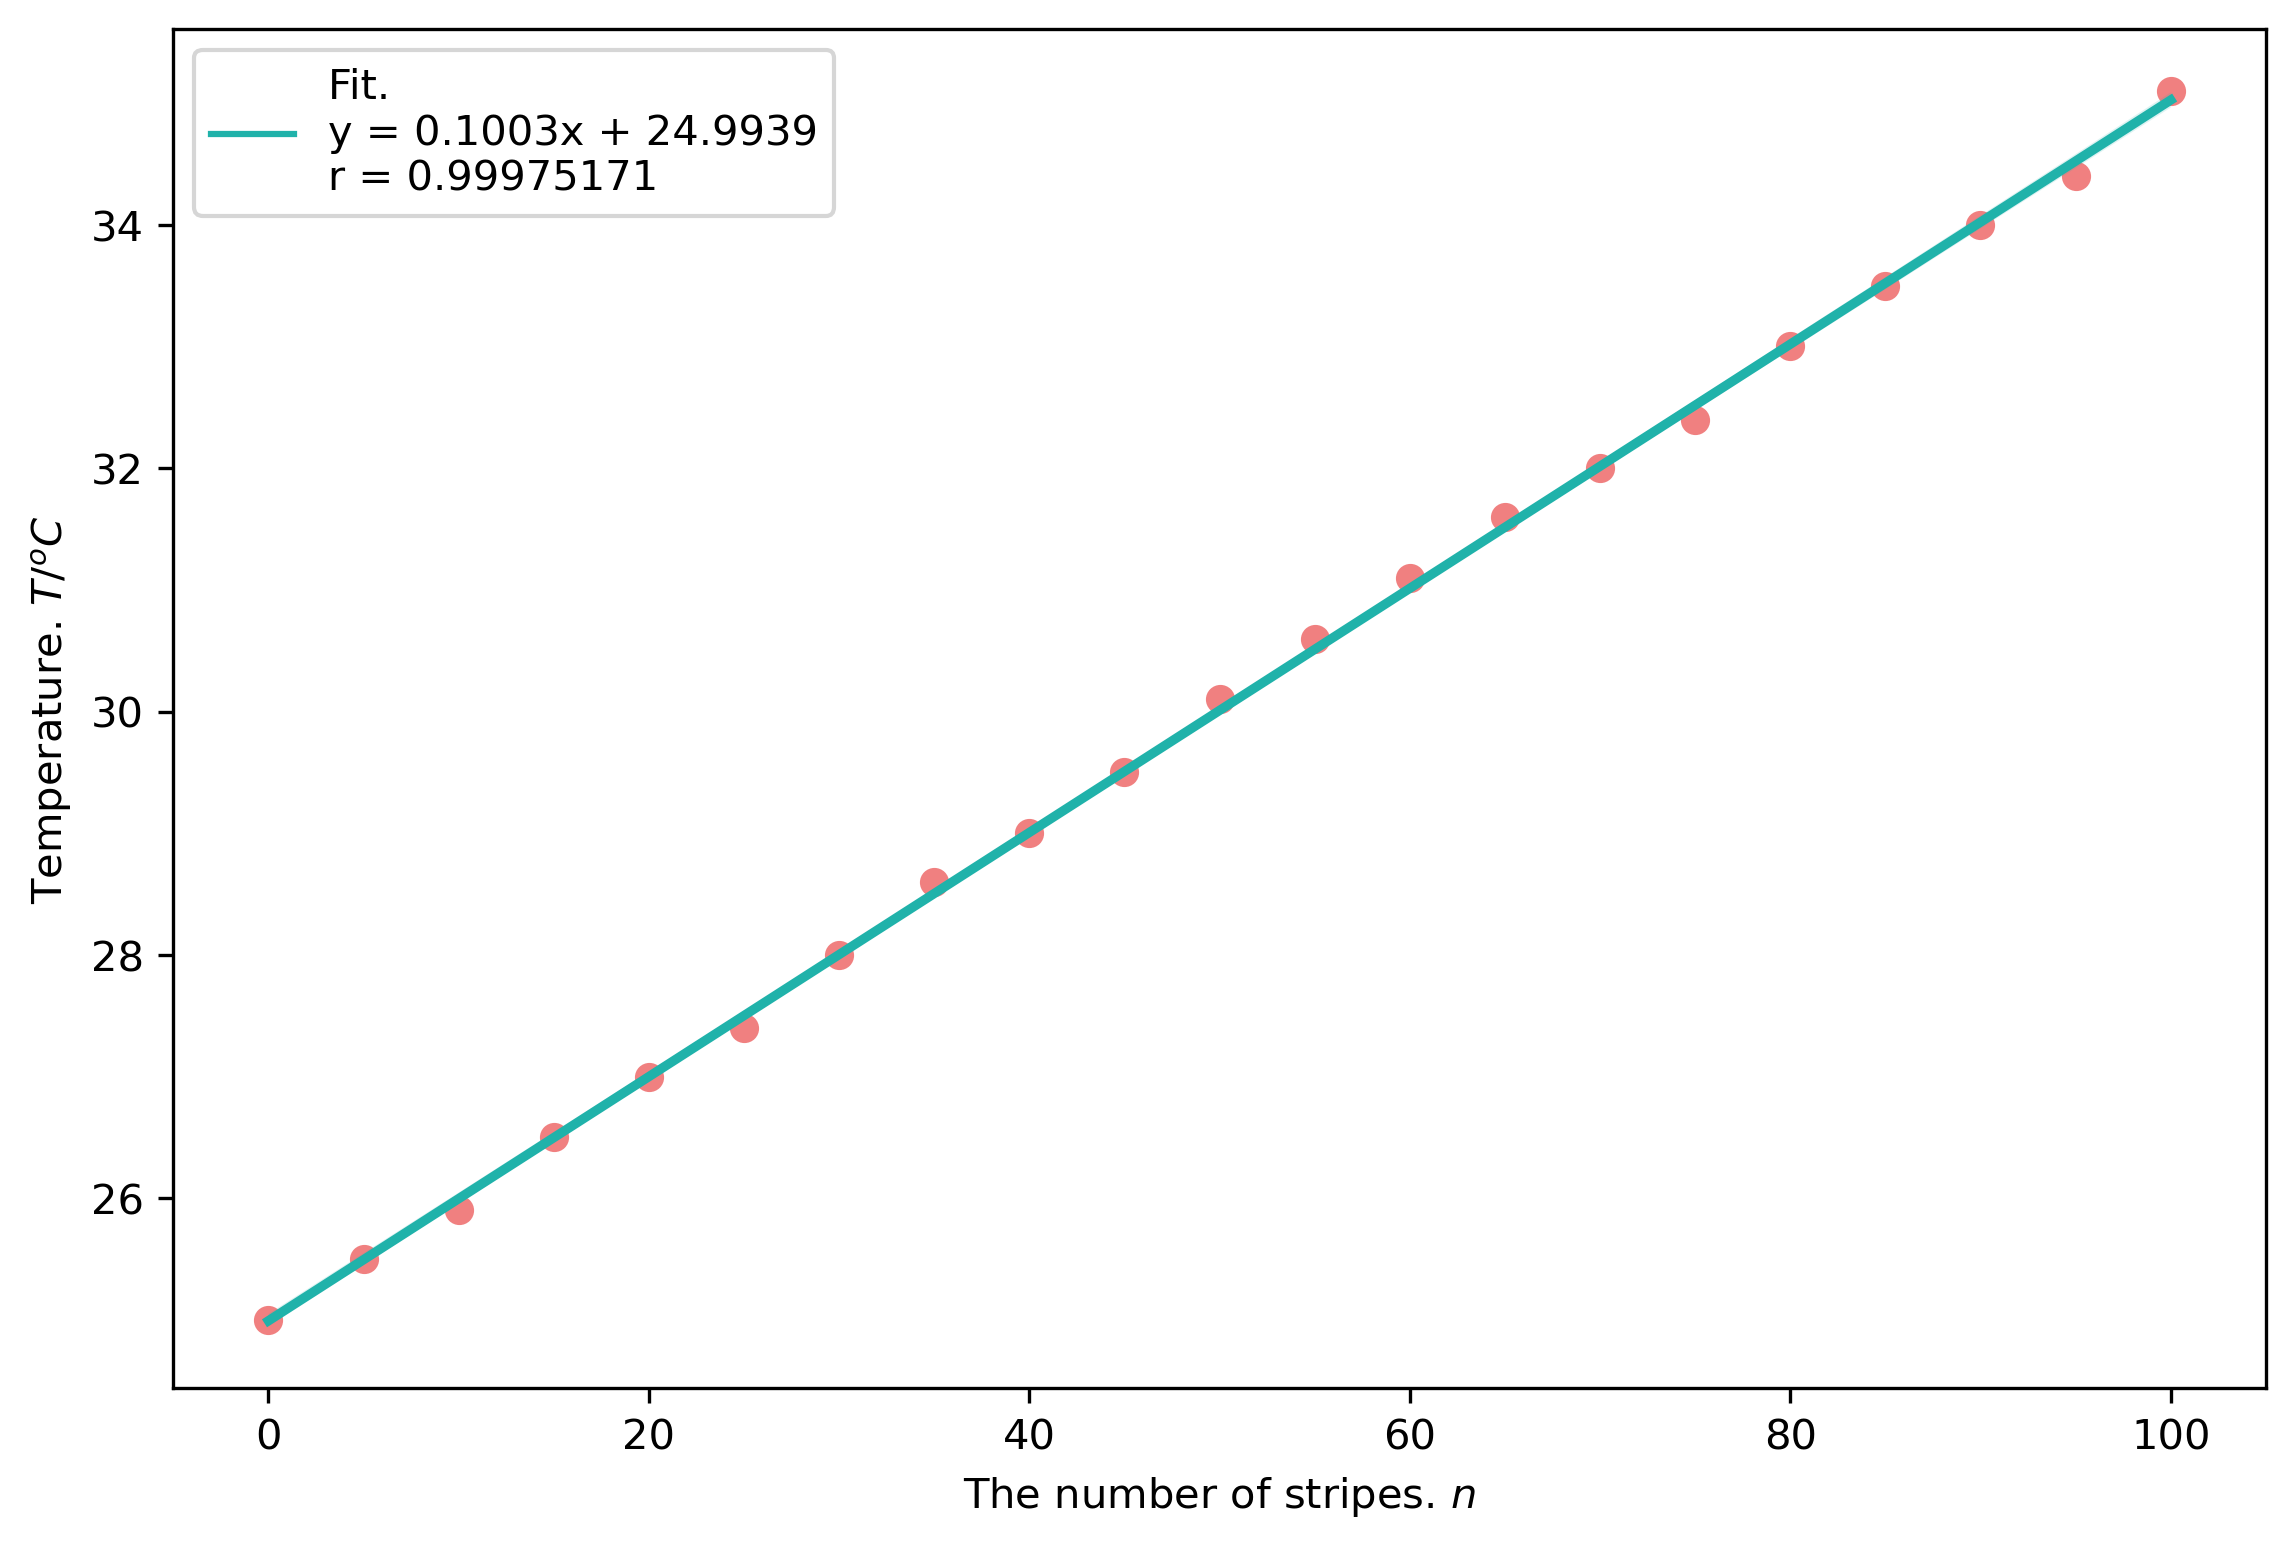
\includegraphics[width=0.4\textwidth]{attachments/fig.2.2.1.2.png}
		}

		\subfloat[2nd Temperature decrease]{\label{fig.2.2.2.1}
		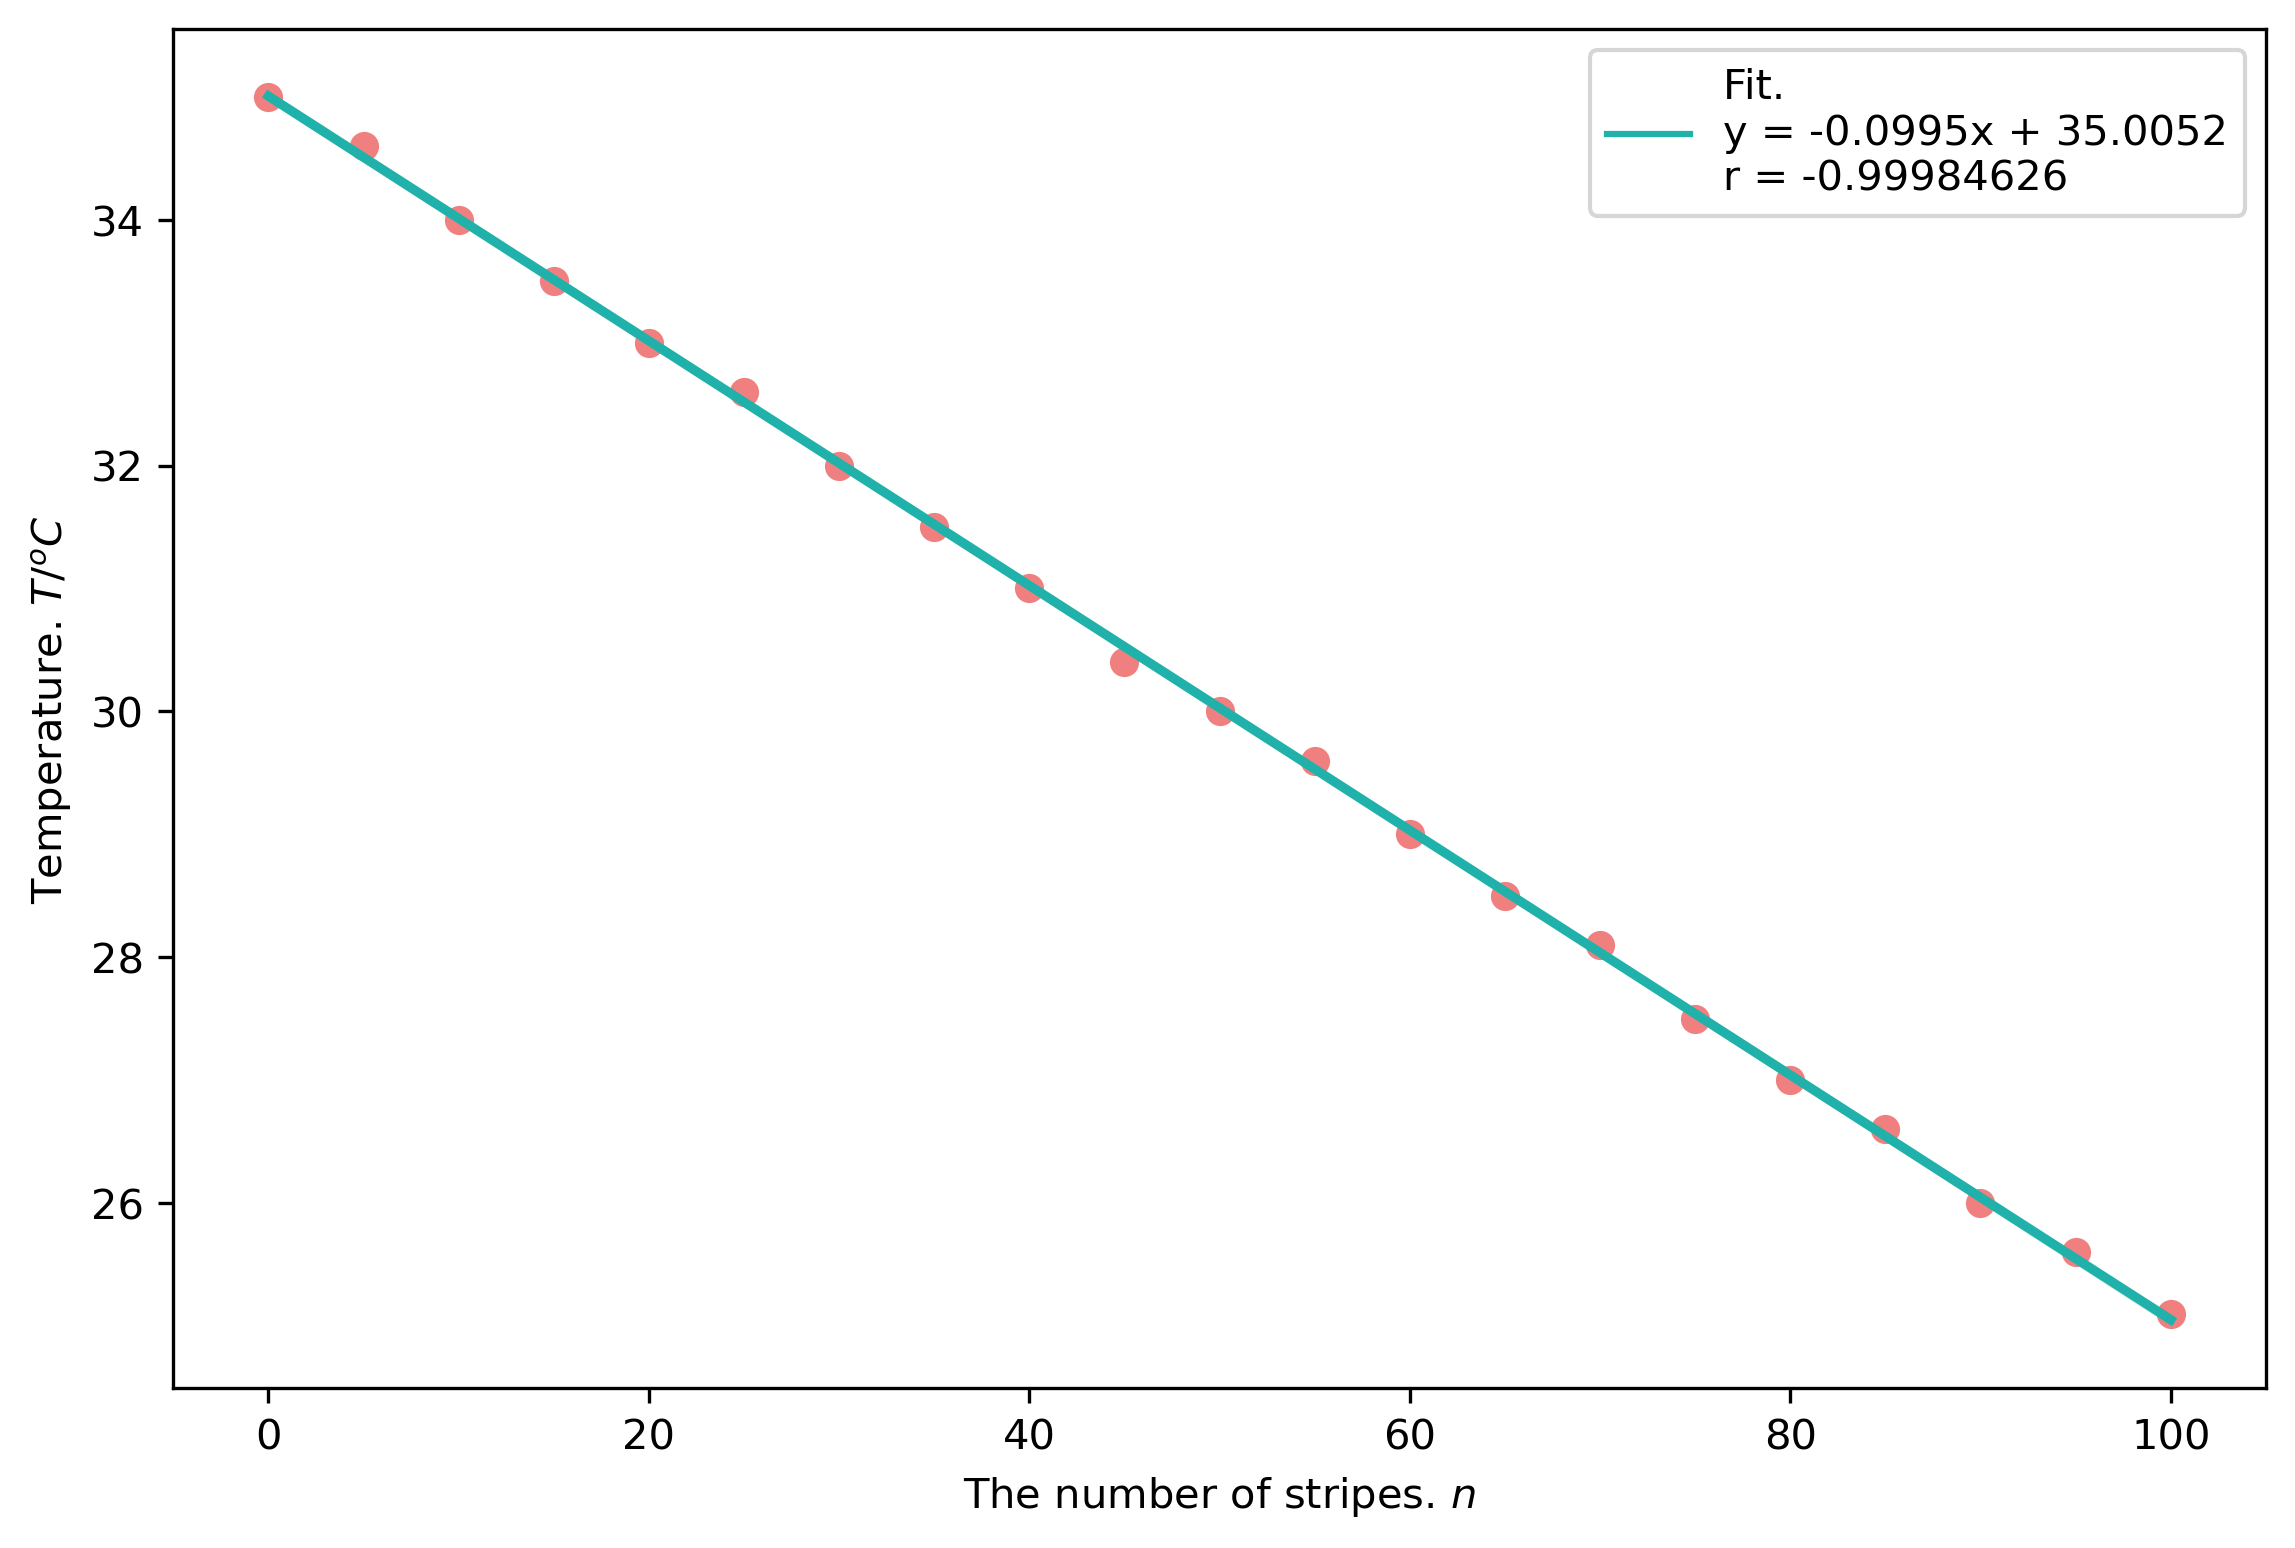
\includegraphics[width=0.4\textwidth]{attachments/fig.2.2.2.1.png}
		}
		\subfloat[2nd Temperature increase]{\label{fig.2.2.2.2}
		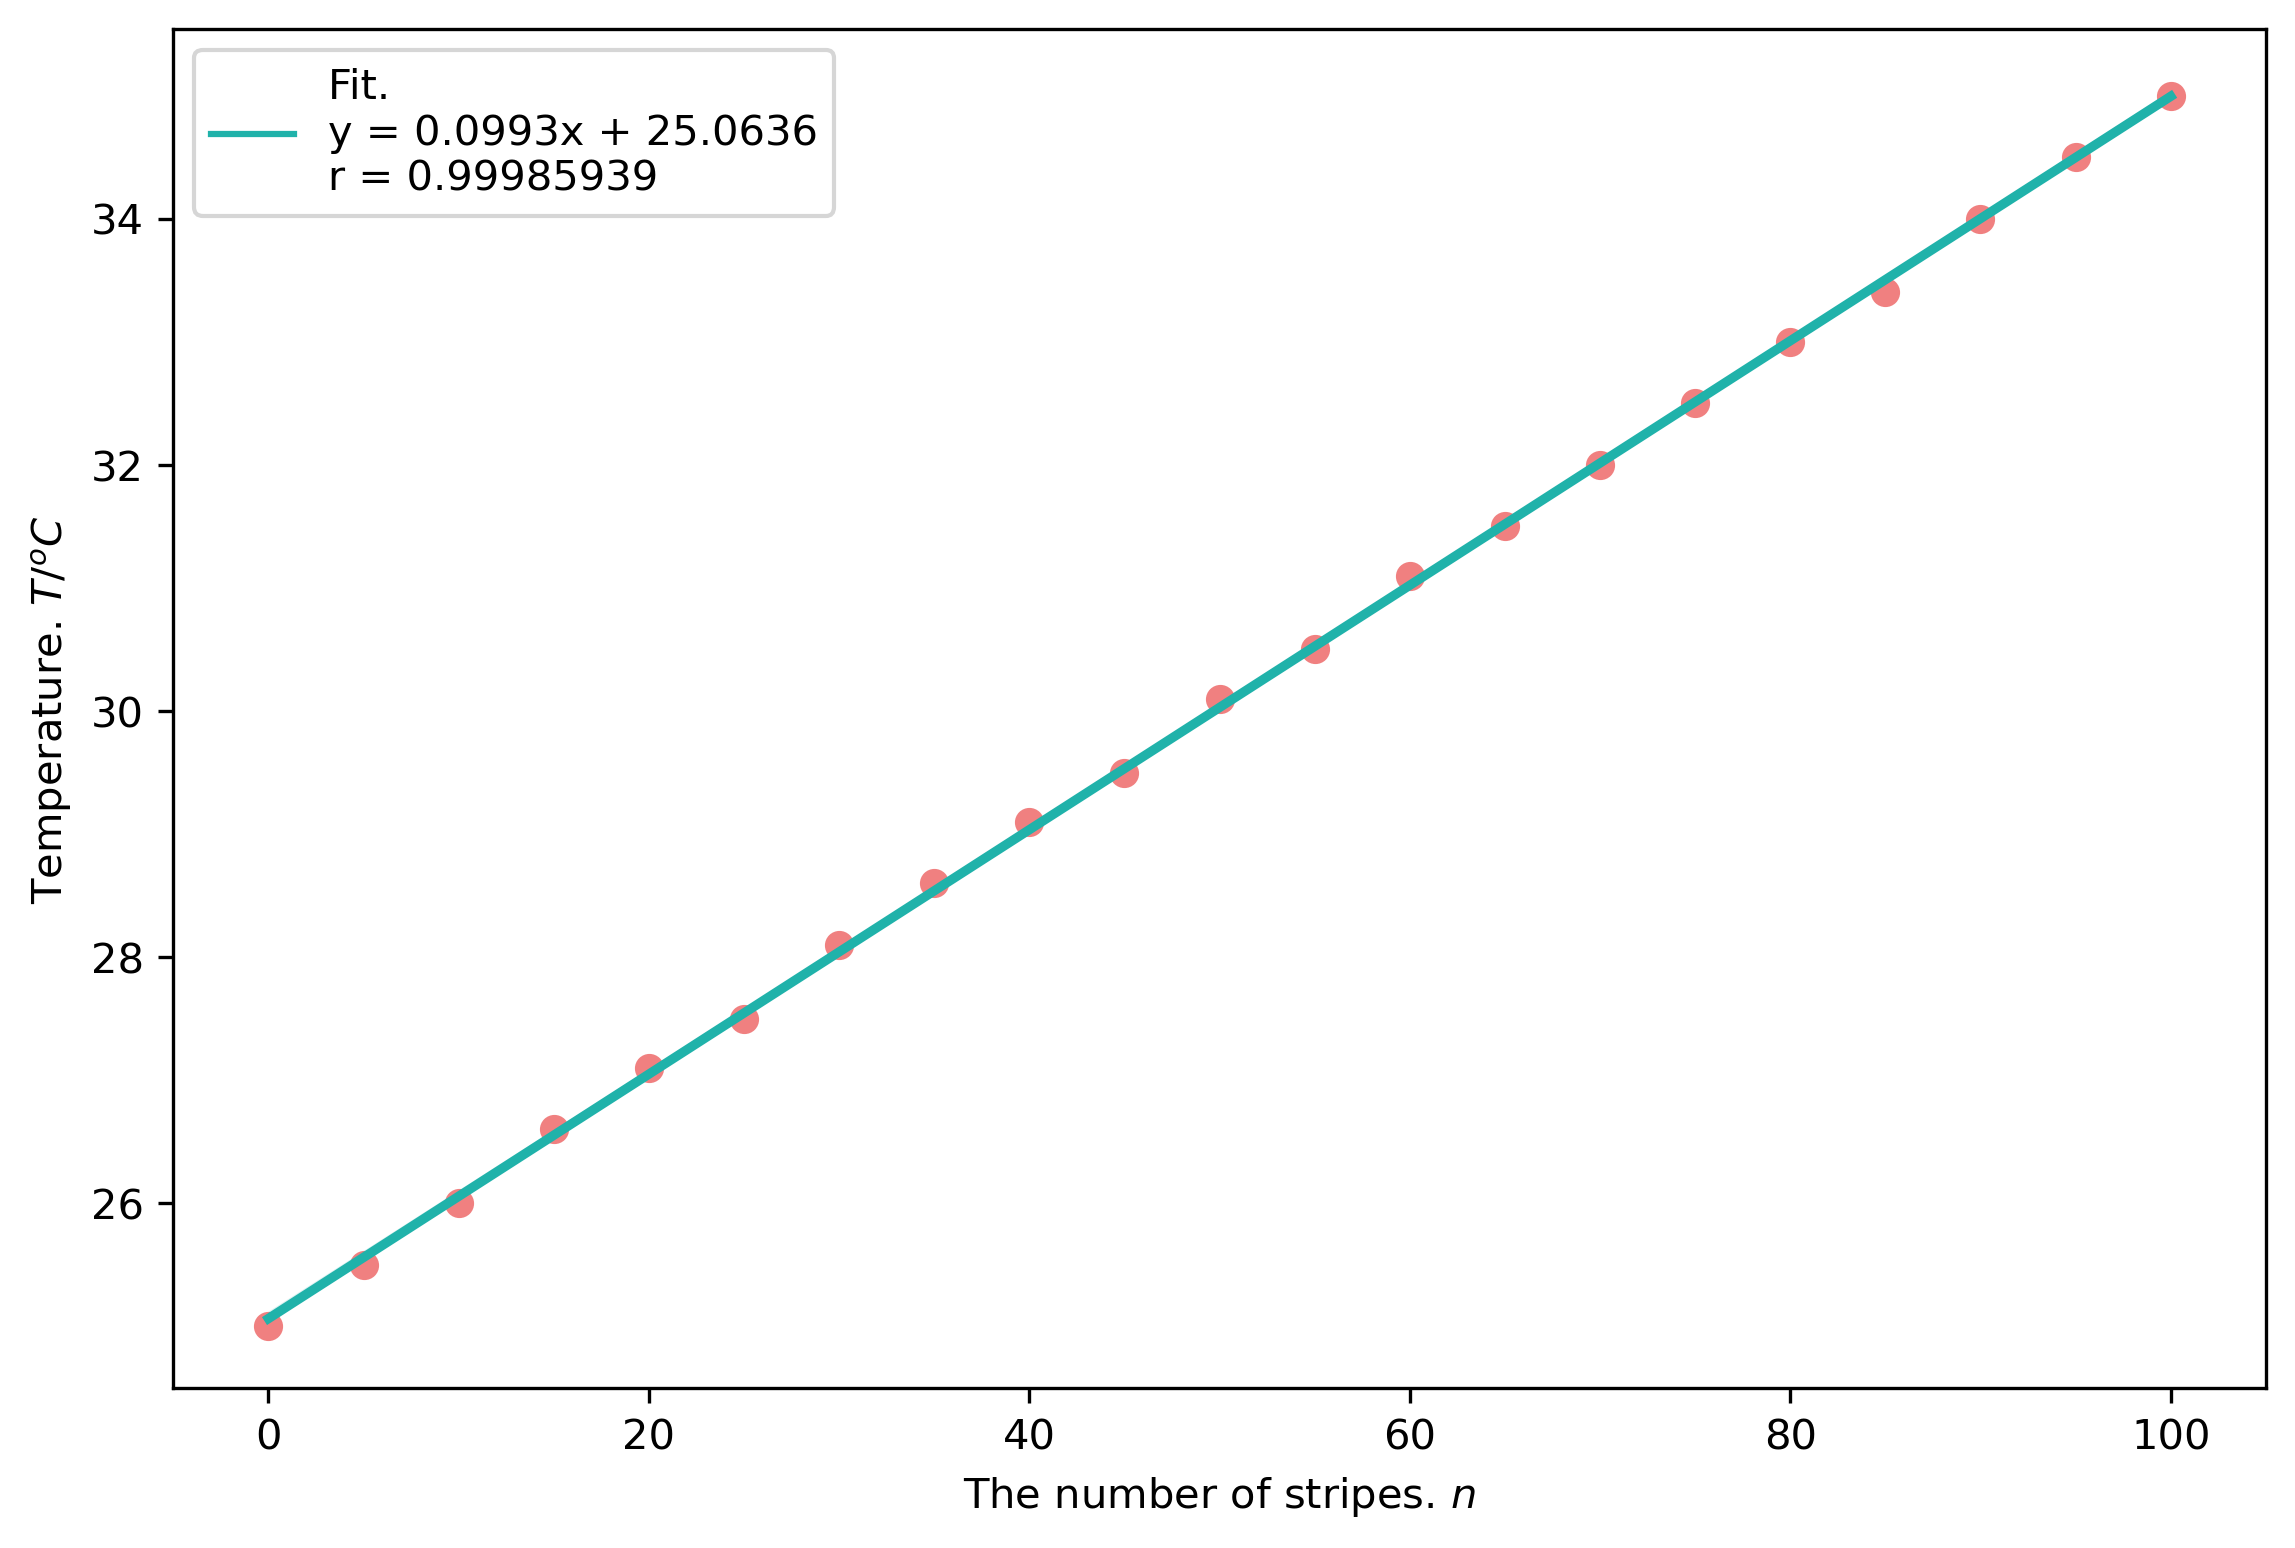
\includegraphics[width=0.4\textwidth]{attachments/fig.2.2.2.2.png}
		}
		\caption{\textbf{Temperature sensor}}
		\label{fig.2.2}
	\end{figure*}
	
	
	For each sensor, we tested twice and the results were almost consistent. We found that the count of shift of the interference fringes increase or decrease linearly as the strain or temperature change.
	According to Eq. \ref{eq.6.1} and Eq. \ref{eq.6.2}, which are obviously not univariate linear functions, 
	we suppose that the reason is that changes of the strain and temperature in our experiment were both not to large that other items in the equation can be ignored; that is, the instrument was working in the linear zone.
	Taking advantage of this property, measuring tiny changes of the strain or temperature using these sensors can be very precious.
	
	The quantitative relationships between the measurand and the count of shift of the interference fringes have been plotted in the corresponding figures.

%%end-------------------Result-----------------------%%

%%begin-------------------Conclusion and Discussion-----------------------%%
\section{Conclusion and Discussion}
	\subsection{Conclusion}
	In this experiment we investigated the optical properties of optical fibers including the coupling efficiency, the numerical aperture, and its effect on the polarization state of the light, 
	and developed high-precision pressure and temperature sensors based on the optical fiber-based Mach-Zehnder interferometer.
	We proved that coupling through a lens could gain an impressive great improvement of the coupling efficiency comparing to direct coupling.
	We also discovered that generally fibers with higher diameters tended to have larger numerical apertures and their exit spots were generally more diffused, 
	while fibers with lower diameters tended to have smaller numerical apertures and their exit spots generally showed a concentrated pattern with high light intensity in the center and blurred edges.
	Although unfortunately we cannot yet be able to investigate the impact of fiber transmission on the polarization state of the light, we proved that the Stocks parameters are effective representation of the polarization state.
	We finally developed high-precision strain and temperature sensors based on the optical-fiber-based Mach-Zehnder interferometer and found that they reach high stability and precision in the linear zone.
	Our work has provided a deeper insight into the optical fibers and may be of assistance to a wider application of the optical fibers.

	\subsection{Known limitation}
	\subsubsection{Coupling loss}
	In the experiment the highest coupling efficiency we have reached is arround 70\%, which is still not ideal enough. The major deviations include:
	\begin{enumerate}[label=\arabic*.]
		\item Lateral deviation: Deviation due to mismatch between the center of the facula and the center of the fiber
		\item Longitudinal offset: Deviation due to the focus point not on the face of the fiber
		\item Angular deviation: Deviation due to misalignment of the beam and the fiber axis
	\end{enumerate}
	Although with the assistance of the five-dimensional alignment jig, it is still difficult to reach the best position by manual adjustment.
	
	Other factors include the mismatch of the mode of the laser and the mode of the fiber, and the shape of the Gaussian surface of the laser.
	\subsubsection{The numerical aperture}
	\begin{enumerate}[label=\arabic*.]
		\item The shape of the facula was slightly not a perfect round, which made it difficult to determine the accurate diameter.
		\item The edge of the facula was blurry, especially in the single-mode fiber($\phi \ 4\mu m$  and $\phi \ 9\mu m$), which made it difficult to determine the accurate diameter.
	\end{enumerate}
	\subsubsection{The polarization state of the light}
	\begin{enumerate}[label=\arabic*.]
		\item The power of the laser we used was not stable, leading to difficulty and inaccuracy in measuring the light power. When measuring the light power after fiber transmission, this problem was even so prominent that we could not conduct the experiment.
	\end{enumerate}
	
	\subsubsection{The sensor}
	\begin{enumerate}[label=\arabic*.]
		\item For unknown reasons, the fringes were keeping oscillating, which made it difficult to judge the shifting of the fringes.
		\item The precision of the thermometer is not high enough that we could not obtain the actual temperature when certain amounts of fringes pass by.
	\end{enumerate}
	
%%end-------------------Conclusion and Discussion-----------------------%%

%%end--------------------Reference------------------------%%
\printbibliography[title=Reference] 
%%end--------------------Reference------------------------%%
\end{document}